%函数的连续性
\documentclass[main.tex]{subfiles}                                    

\begin{document}
\clearpage

\section{引言}

本章的第 2 到 5 节涵盖了四种表面类型的 NURBS 表示:双线性表面、一般圆柱体(挤压表面)、规则表面和旋转表面。正如读者现在肯定意识到的，这些表示并不是唯一的。参数化、凸包、连续性、软件设计、应用领域、数据交换甚至个人品味等因素都可能影响表示方法的选择。我们的展示紧密跟随 Piegl 和 Tiller [Pieg87a] 提出的构造。第 6 节使用非均匀缩放来获得额外的表面，例如椭球体和椭圆抛物面。第 7 节介绍了一种在球面上构造三边补丁的方法，其边界曲线是半径等于球体半径的圆。这种补丁在作为角落圆角表面时非常有用。

为了清楚地指示本章中的度数，我们使用符号 \({R}_{i,p;j,q}\left( {u,v}\right)\) 表示度数为 \(p \times  q\) 的第 \(i,j\) 个有理基函数(与方程 [4.12] 进行比较)。



\section{双线性曲面}

设 \({\mathbf{P}}_{0,0},{\mathbf{P}}_{1,0},{\mathbf{P}}_{0,1},{\mathbf{P}}_{1,1}\) 为三维空间中的四个点。我们希望构造通过在四条线段之间进行双线性插值而获得的曲面的 NURBS 表示， \({\mathbf{P}}_{0,0}{\mathbf{P}}_{1,0},{\mathbf{P}}_{0,1}{\mathbf{P}}_{1,1},{\mathbf{P}}_{0,0}{\mathbf{P}}_{0,1}\) 和 \({\mathbf{P}}_{1,0}{\mathbf{P}}_{1,1}.\) 显然，所需的(非有理)曲面由以下公式给出

\[
\mathbf{S}\left( {u,v}\right)  = \mathop{\sum }\limits_{{i = 0}}^{1}\mathop{\sum }\limits_{{j = 0}}^{1}{N}_{i,1}\left( u\right) {N}_{j,1}\left( v\right) {\mathbf{P}}_{i,j} \tag{8.1}
\]

其中

\[
U = V = \{ 0,0,1,1\}
\]

方程 (8.1) 表示在两个方向上相对边界线之间的简单线性插值。在图 8.1a 中，四个点位于同一平面内，因此曲面是由四条线段所界定的平面的一部分。图 8.1b 显示了通过在立方体的非平行对角线之间进行线性插值得到的双曲抛物面。



\section{一般圆柱体}

设 \(\mathbf{W}\) 为单位长度的向量， \(\mathbf{C}\left( u\right)  = \mathop{\sum }\limits_{{i = 0}}^{n}{R}_{i,p}\left( u\right) {\mathbf{P}}_{i}\) 为节点向量 \(U\) 上的 \(p\) 次 NURBS 曲线，权重为 \({w}_{i}\) 。我们希望得到通过沿 \(\mathbf{W}\) 方向以距离 \(d\) 进行扫掠而获得的一般圆柱体 \(\mathbf{S}\left( {u,v}\right)\) 的表示。用 \(v,0 \leq  v \leq  1\) 表示扫掠方向的参数，显然 \(\mathbf{S}\left( {u,v}\right)\) 必须满足两个条件

\begin{itemize}
\item 对于固定的 \(\bar{u},\mathbf{S}\left( {\bar{u},v}\right)\) ，是从 \(\mathbf{C}\left( \bar{u}\right)\) 到 \(\mathbf{C}\left( \bar{u}\right)  + d\mathbf{W}\) 的一条直线段；
\end{itemize}

\begin{itemize}
\item 对于固定的 \(\bar{v}\)
\end{itemize}

\[
\mathbf{S}\left( {u,\bar{v}}\right)  = \mathbf{C}\left( u\right)  + \bar{v}d\mathbf{W} = \mathop{\sum }\limits_{{i = 0}}^{n}{R}_{i,p}\left( {{\mathbf{P}}_{i} + \bar{v}d\mathbf{W}}\right)
\]

(平移不变性属性)。

所需的表示为

\[
\mathbf{S}\left( {u,v}\right)  = \mathop{\sum }\limits_{{i = 0}}^{n}\mathop{\sum }\limits_{{j = 0}}^{1}{R}_{i,p;j,1}\left( {u,v}\right) {\mathbf{P}}_{i,j} \tag{8.2}
\]

在节点向量 \(U\) 和 \(V\) 上，其中 \(V = \{ 0,0,1,1\}\) 和 \(U\) 是 \(\mathbf{C}\left( u\right)\) 的节点向量。控制点由 \({\mathbf{P}}_{i,0} = {\mathbf{P}}_{i}\) 和 \({\mathbf{P}}_{i,1} = {\mathbf{P}}_{i} + d\mathbf{W}\) 给出，权重为 \({w}_{i,0} = {w}_{i,1} = {w}_{i}\) 。图 8.2 显示了一般圆柱体。

右圆柱体是通过将 NURBS 圆沿与圆平面法向的向量平移距离 \(d\) 得到的。第 7 章中给出的任何圆的表示方式都可以使用。图 8.3 显示了一个右圆柱体，其底层圆是示例 Ex7.2 和图 7.16a 的二次九点方形控制多边形表示。该圆柱体由以下公式定义

\[
\mathbf{S}\left( {u,v}\right)  = \mathop{\sum }\limits_{{i = 0}}^{8}\mathop{\sum }\limits_{{j = 0}}^{1}{R}_{i,2;j,1}\left( {u,v}\right) {\mathbf{P}}_{i,j} \tag{8.3}
\]

其中 \(V = \{ 0,0,1,1\}\) 和 \(U\) ，权重 \(\left( {w}_{i,0}\right.\) 和 \(\left. {w}_{i,1}\right)\) 是示例 Ex7.2 中给出的圆的权重。注意，控制网形成了圆柱体的外接框。

通过平移由算法 A7.1 和 A7.3 计算出的控制点，可以获得横截面为圆形和锥形且扫掠角小于 \({360}^{ \circ  }\) 的圆柱体。图 8.4 显示了一个椭圆柱体。

\begin{center}
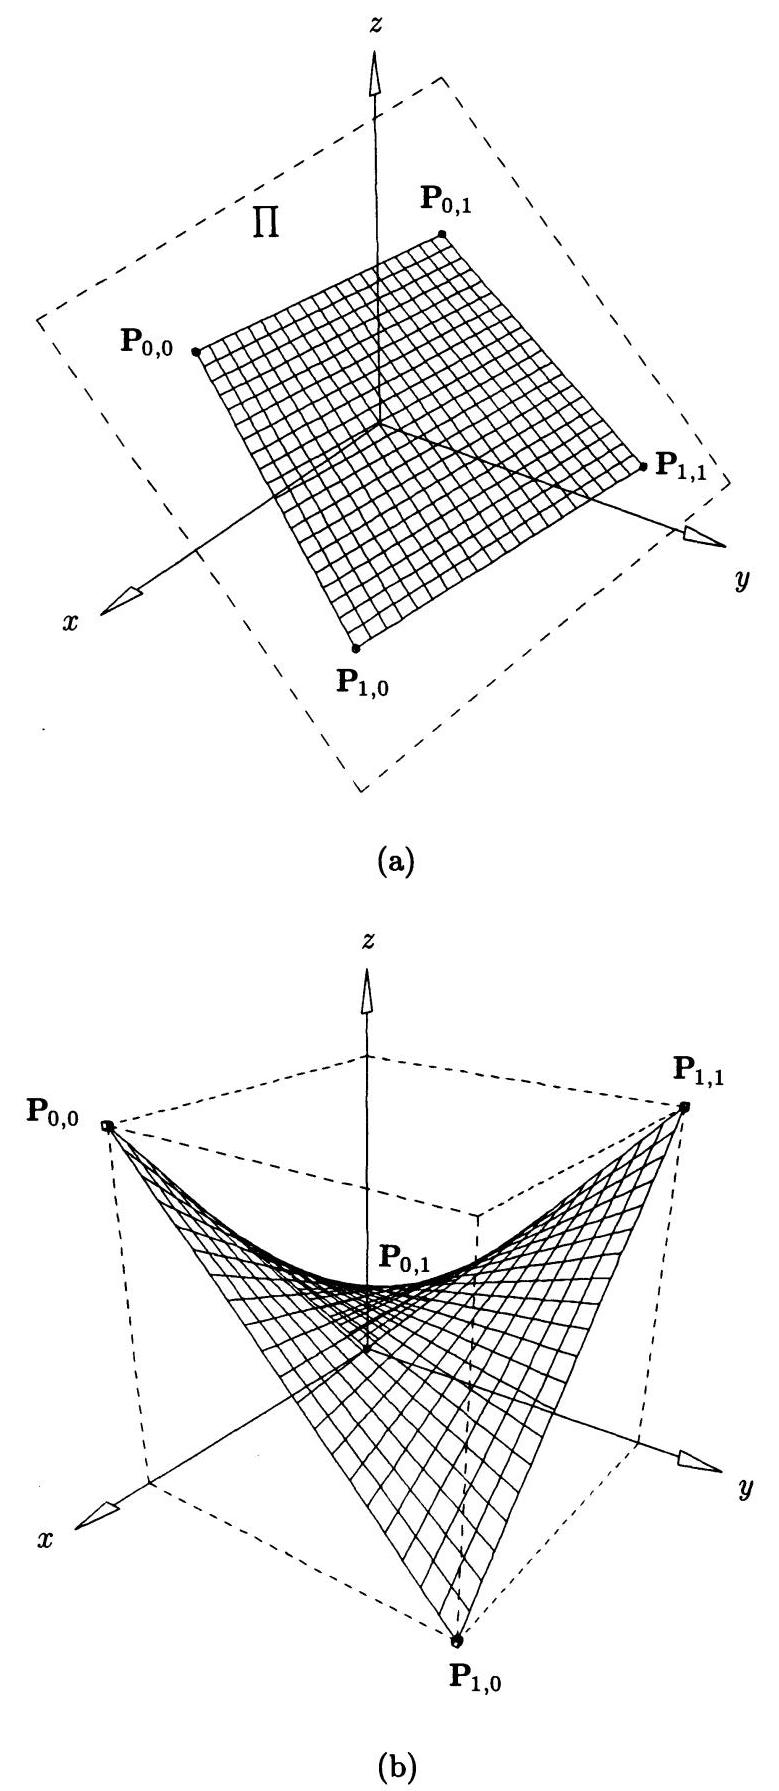
\includegraphics[max width=0.7\textwidth]{images/0193ba0d-ab19-7138-9798-cb281ce60de0_342_379_249_779_1791_0.jpg}
\end{center}
\hspace*{3em} 

图 8.1. 双线性曲面。(a) 位于平面 \(\Pi\) 的直线边界；(b) 非平面直线边界(由立方体的对角线定义)形成双曲抛物面。

336 常见曲面的构造

\begin{center}
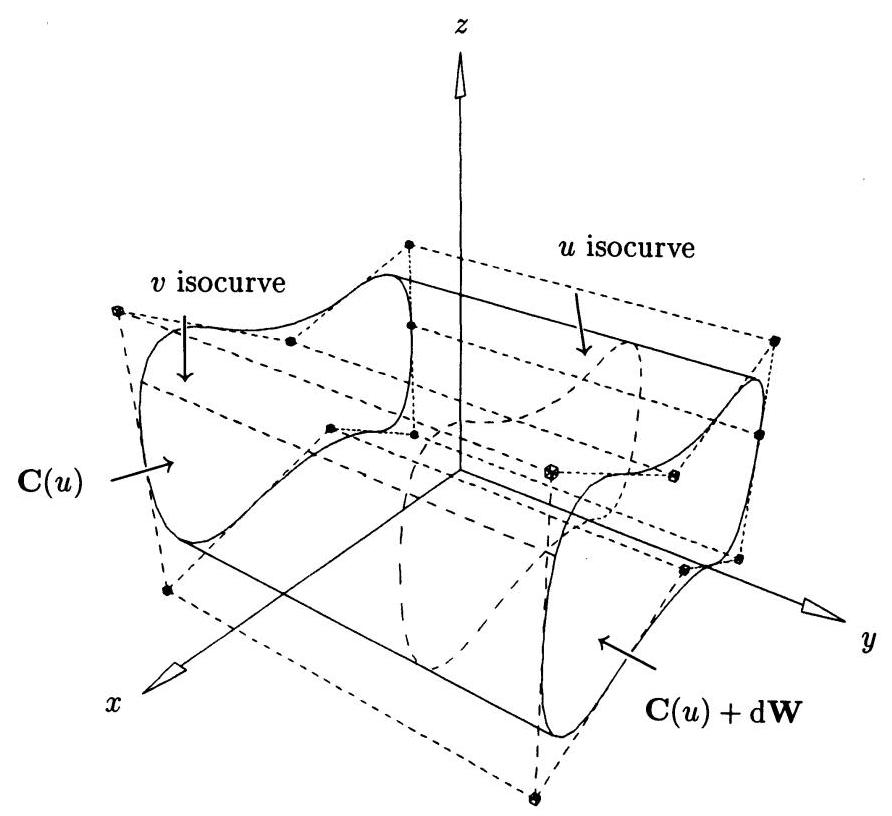
\includegraphics[max width=0.8\textwidth]{images/0193ba0d-ab19-7138-9798-cb281ce60de0_343_351_246_892_816_0.jpg}
\end{center}
\hspace*{3em} 

图 8.2. 通过沿 \(\mathbf{W}\) 平移距离 \(d\) 得到的一般圆柱体。

\begin{center}
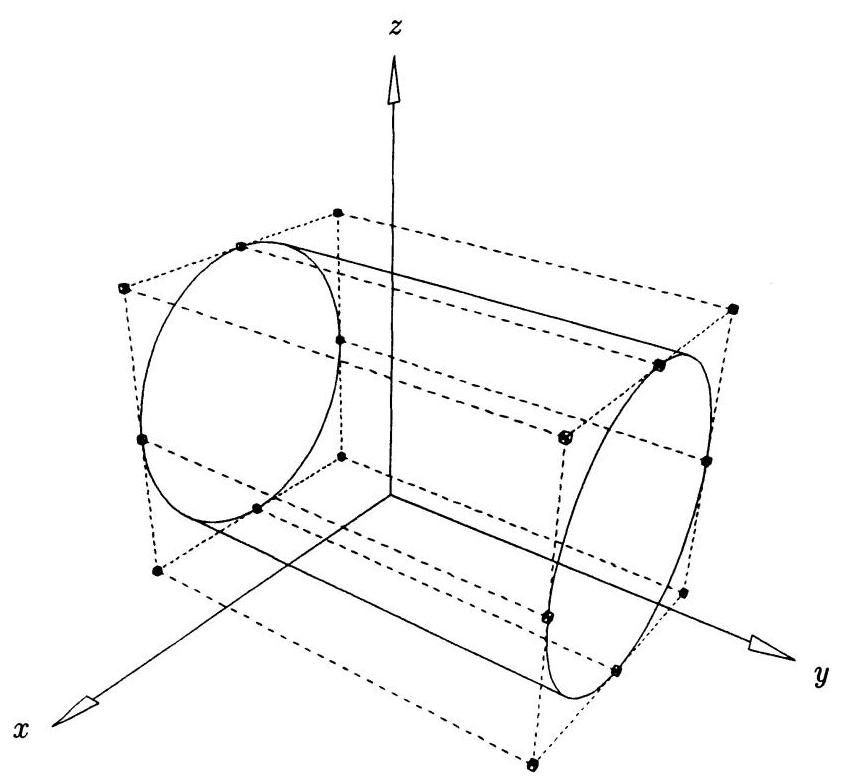
\includegraphics[max width=0.7\textwidth]{images/0193ba0d-ab19-7138-9798-cb281ce60de0_343_371_1299_841_783_0.jpg}
\end{center}
\hspace*{3em} 

图 8.3. 右圆柱体。

\begin{center}
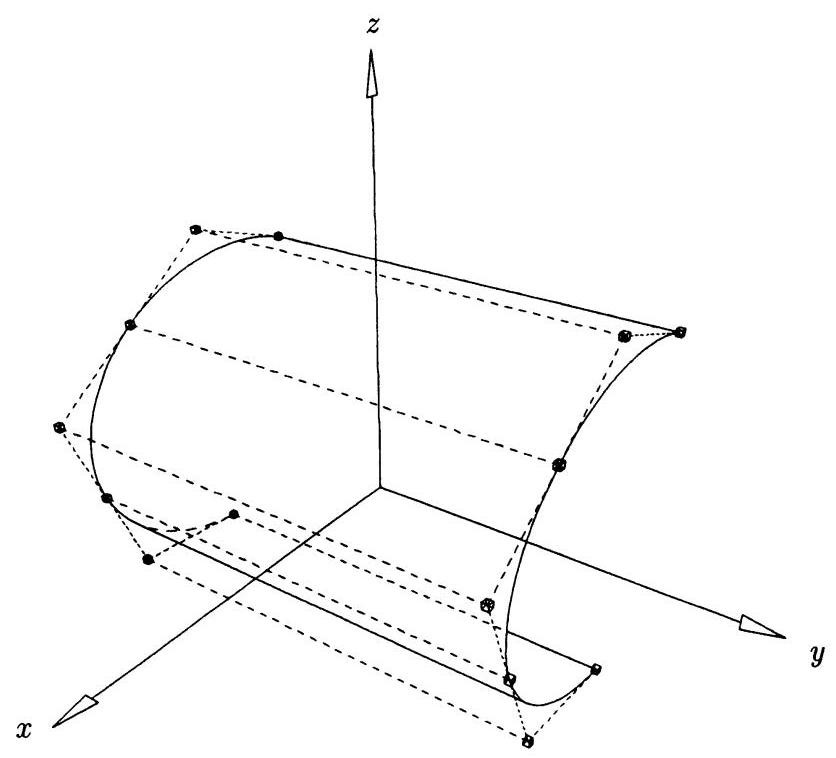
\includegraphics[max width=0.7\textwidth]{images/0193ba0d-ab19-7138-9798-cb281ce60de0_344_344_260_836_758_0.jpg}
\end{center}
\hspace*{3em} 

图 8.4. 椭圆柱面片。


\section{规则曲面}

假设我们有两个 NURBS 曲线

\[
{\mathbf{C}}_{k}\left( u\right)  = \mathop{\sum }\limits_{{i = 0}}^{{n}_{k}}{R}_{i,{p}_{k}}\left( u\right) {\mathbf{P}}_{i}^{k}\;k = 1,2
\]

定义在结点向量 \({U}^{k} = \left\{  {{u}_{0}^{k},\ldots ,{u}_{{m}_{k}}^{k}}\right\}\) 上。我们希望得到一个在 \(v\) 方向上被规则化的曲面，即它是 \({\mathbf{C}}_{1}\left( u\right)\) 和 \({\mathbf{C}}_{2}\left( u\right)\) 之间的线性插值。此外，我们要求插值在相同参数值的点之间进行，即，对于固定的 \(\bar{u},\mathbf{S}\left( {\bar{u},v}\right)\) ，它是连接点 \({\mathbf{C}}_{1}\left( \bar{u}\right)\) 和 \({\mathbf{C}}_{2}\left( \bar{u}\right)\) 的直线段。所需的曲面形式是

\[
\mathbf{S}\left( {u,v}\right)  = \mathop{\sum }\limits_{{i = 0}}^{n}\mathop{\sum }\limits_{{j = 0}}^{1}{R}_{i,p;j,1}\left( {u,v}\right) {\mathbf{P}}_{i,j} \tag{8.4}
\]

其中 \(V = \{ 0,0,1,1\} .n,U,p,{w}_{i,j}\) ，并且 \({\mathbf{P}}_{i,j}\) 必须全部确定。

由于曲面的张量积特性，两个边界曲线 \({\mathbf{C}}_{k}\left( u\right)\) 必须具有相同的度，并且定义在相同的结点向量上。因此，确定 \(n,U,p,{w}_{i,j}\) 和 \({\mathbf{P}}_{i,j}\) 的算法是

1. 确保两个曲线定义在相同的参数范围内，即，

\[
{u}_{0}^{1} = {u}_{0}^{2}\text{ and }{u}_{{m}_{1}}^{1} = {u}_{{m}_{2}}^{2}
\]

2. 如果 \({p}_{1} = {p}_{2}\) ，则设置 \(p = {p}_{1}\) ；否则，将 \(p\) 设置为 \({p}_{1},{p}_{2}\) 中的较大值，并将较低度曲线的度提升到 \(p\) (算法 A5.9)；

3. 如果结点向量 \({U}^{1}\) 和 \({U}^{2}\) 不相同，则合并它们以获得结点向量 \(U\) ；更准确地说，如果 \({u}_{j}\) 在 \({U}^{1}\) 或 \({U}^{2}\) 中，则它在 \(U\) 中。 \({u}_{j}\) 在 \({U}^{1}\) 或 \({U}^{2}\) 中的最大重数也会转移到 \(U\) 。例如，如果 \({U}^{1} = \{ 0,0,0,1,2,2,4,4,4\}\) 和 \({U}^{2} = \{ 0,0,0,1,2,3,4,4,4\}\) ，则 \(U = \{ 0,0,0,1,2,2,3,4,4,4\}\) ；

4. 使用 \(U\) ，对两个曲线 \({\mathbf{C}}_{k}\left( u\right)\) 应用结点细化(算法 A5.4)；此步骤产生 \(n,{w}_{i,j}\) 和 \({\mathbf{P}}_{i,j}\) 的最终值。

图 \({8.5}\mathrm{a} - {8.5}\mathrm{e}\) 显示了在二次曲线和三次曲线之间构造规则曲面的过程。

一般锥体也是一个有规则的曲面。设 \(\mathbf{P}\) 为锥体的顶点，

并设

\[
{\mathbf{C}}_{1}\left( u\right)  = \mathop{\sum }\limits_{{i = 0}}^{n}{R}_{i,p}\left( u\right) {\mathbf{P}}_{i}^{1}
\]

为其基曲线。定义曲线

\[
{\mathbf{C}}_{2}\left( u\right)  = \mathop{\sum }\limits_{{i = 0}}^{n}{R}_{i,p}\left( u\right) {\mathbf{P}}_{i}^{2}
\]

以 \({\mathbf{P}}_{i}^{2} = \mathbf{P}\) 和 \({w}_{i}^{2} = {w}_{i}^{1}\) 为所有 \(i\) (一个退化曲线)。在 \({\mathbf{C}}_{1}\left( u\right)\) 和 \({\mathbf{C}}_{2}\left( u\right)\) 之间的有规则曲面就是所需的锥体。图 8.6 显示了一个直圆锥，图 8.7a-8.7c 显示了一些由直线和圆定义的奇异有规则曲面。

\begin{center}
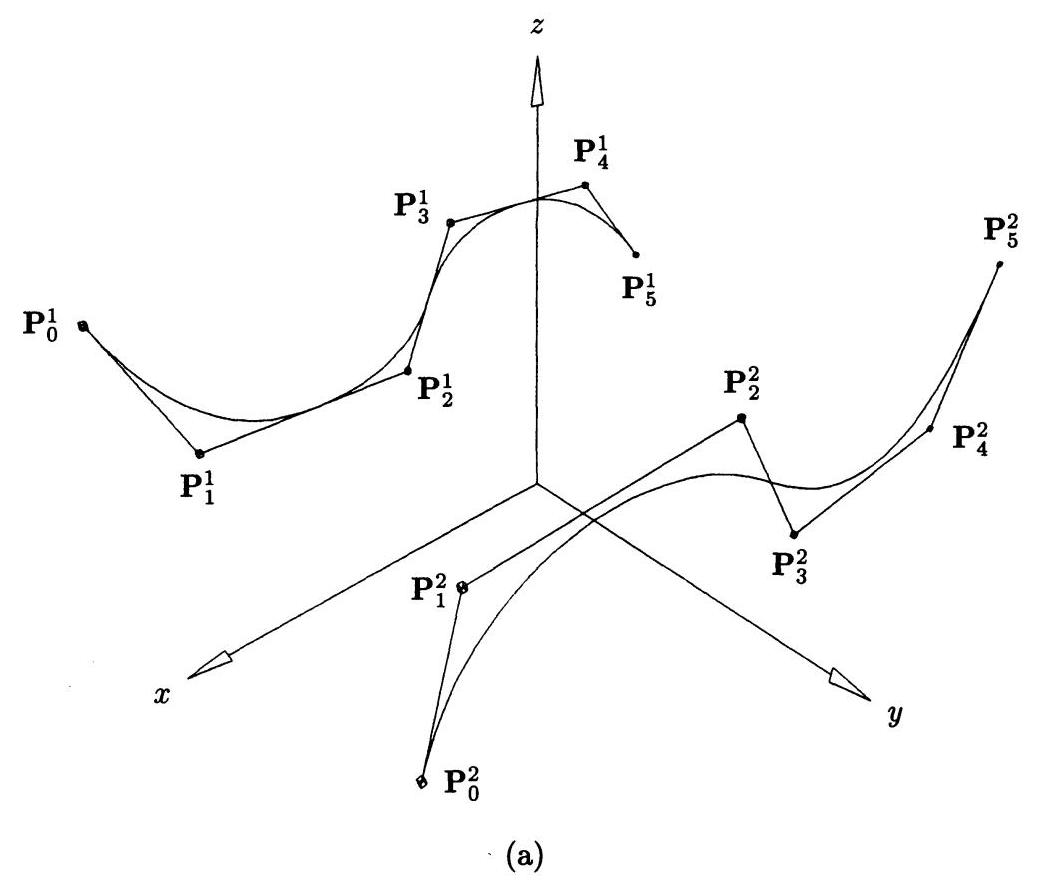
\includegraphics[max width=0.9\textwidth]{images/0193ba0d-ab19-7138-9798-cb281ce60de0_345_249_1148_1040_881_0.jpg}
\end{center}
\hspace*{3em} 

图 8.5. 在两个 NURBS 曲线之间构造有规则曲面。(a)输入的二次和三次曲线， \({U}^{1} = \{ 0,0,0,1/4,1/2,3/4,1,1,1\}\) 和 \({U}^{2} =\)  \(\{ 0,0,0,0,0,3/{10},7/{10},1,1,1\}\) 。

\begin{center}
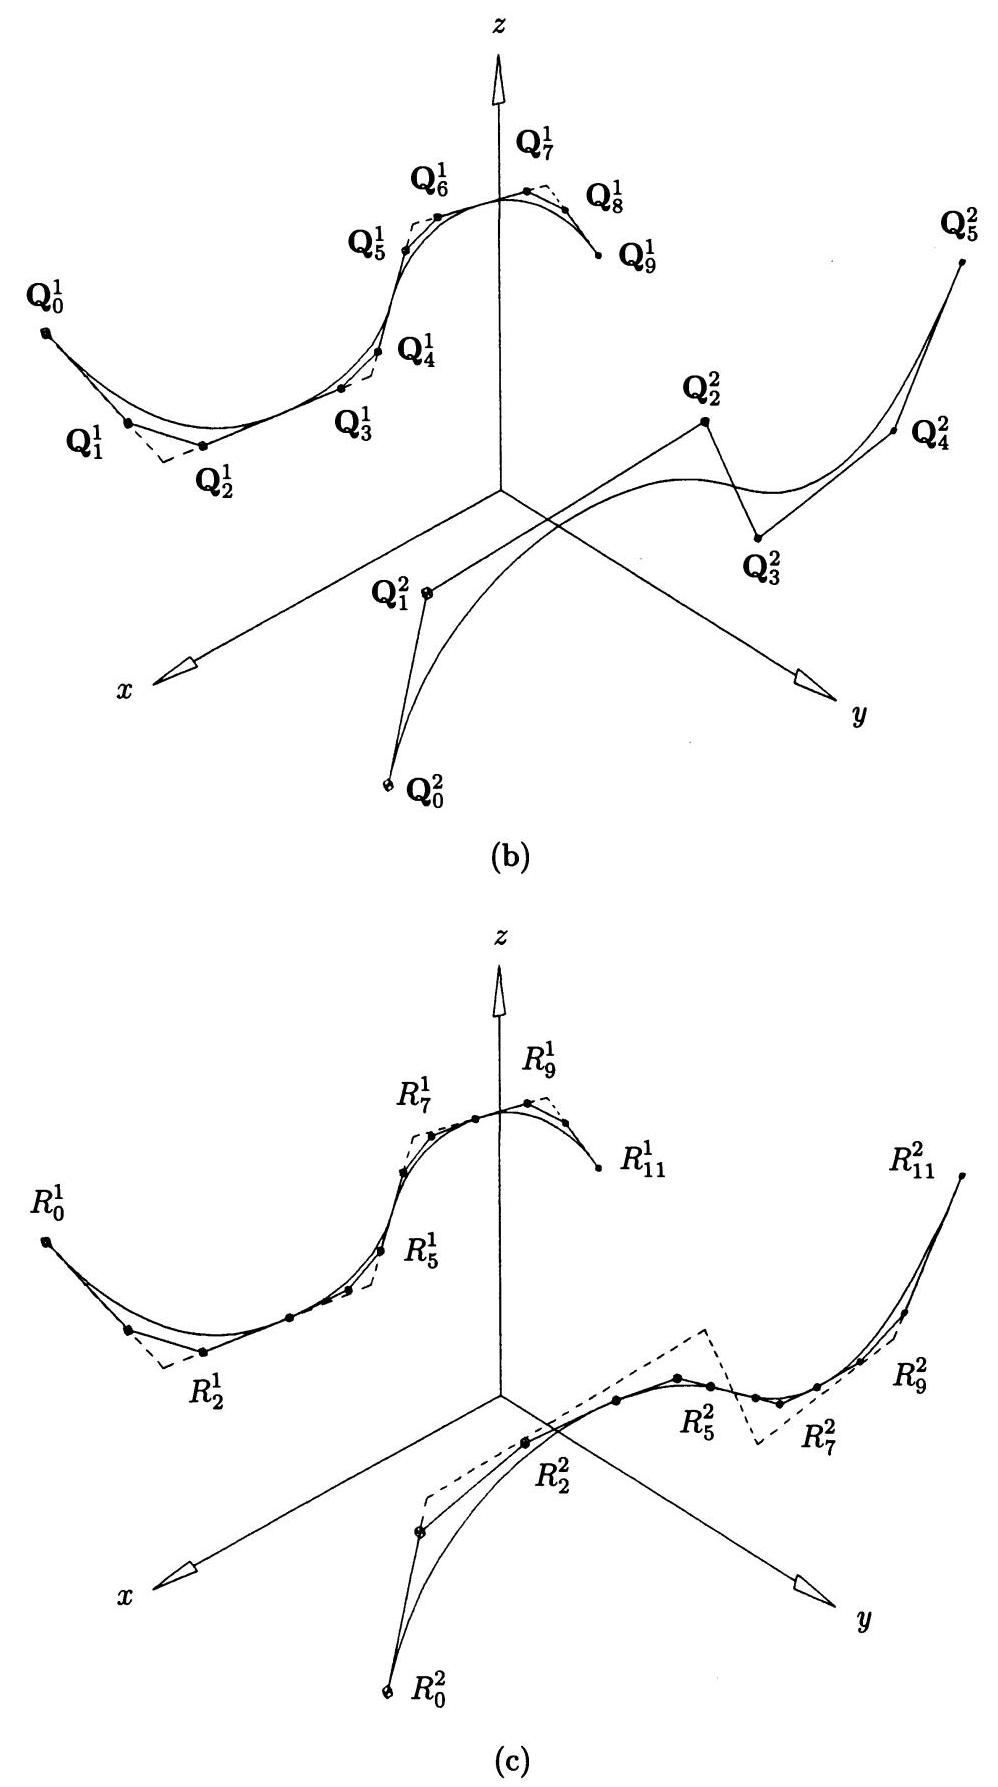
\includegraphics[max width=0.9\textwidth]{images/0193ba0d-ab19-7138-9798-cb281ce60de0_346_263_243_998_1787_0.jpg}
\end{center}
\hspace*{3em} 

图 8.5.(续。)(b) 二次曲线的次数提升；(c) 合并节点向量后的节点精细化曲线；曲面节点向量为 \(U = \{ 0,0,0,0,1/4,1/4,3/{10},\) 。

\(1/2,1/2,7/{10},3/4,3/4,1,1,1,1\}\) .

\begin{center}
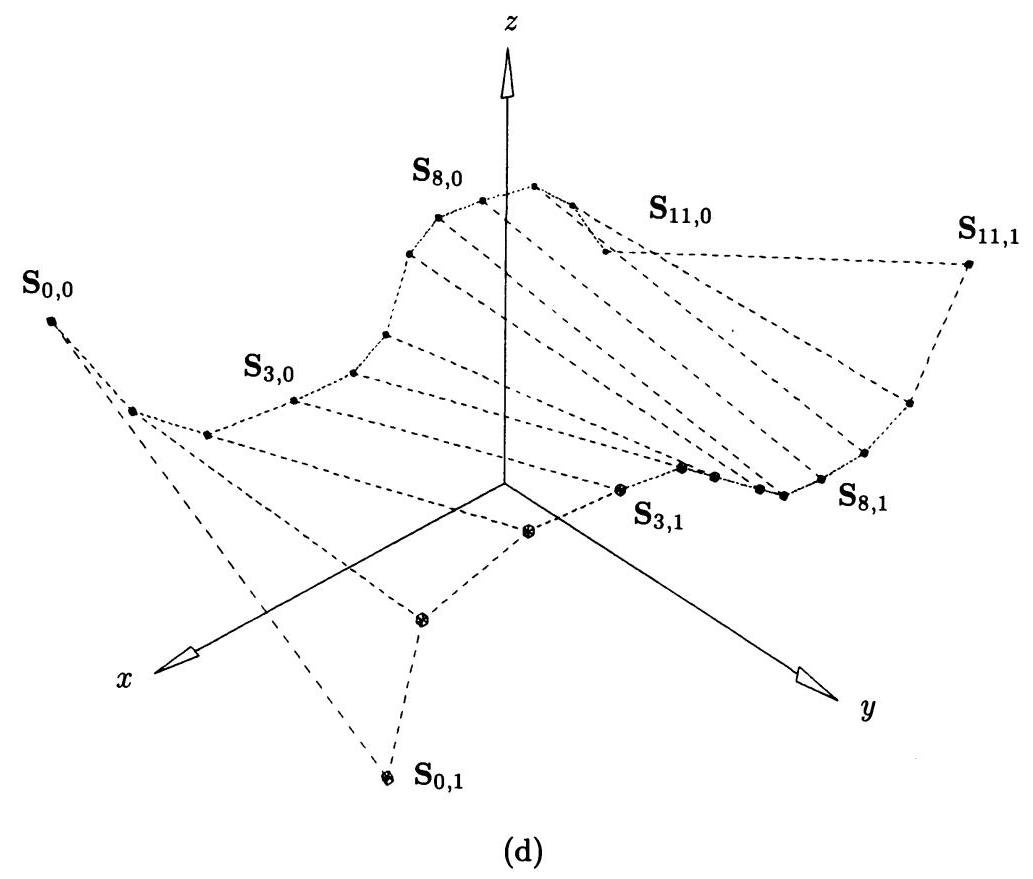
\includegraphics[max width=0.9\textwidth]{images/0193ba0d-ab19-7138-9798-cb281ce60de0_347_253_256_1033_879_0.jpg}
\end{center}
\hspace*{3em} 

图 8.5.(续。)(d) 有规则曲面的控制网。

我们再次强调，NURBS 曲面上的有规则线段(直线段)是在参数值相等的点之间，而不是在相对弧长相等的点之间。一般来说，按照相对弧长进行有规则化会产生几何上不同的曲面，而这无法通过 NURBS 实现。因此，NURBS 与 IGES 有规则曲面(类型 118)，形式 0 [IGE93] 之间的数学精确转换是不可能的。


\section{旋转曲面}
设 \(\mathbf{C}\left( v\right)  = \mathop{\sum }\limits_{{j = 0}}^{m}{R}_{j,q}\left( v\right) {\mathbf{P}}_{j}\) 为在节点向量 \(V\) 上的 \(q\) 阶 NURBS 曲线。 \(\mathbf{C}\left( v\right)\) 被称为生成线，它将围绕一个轴旋转。在本节的最后，我们将介绍一个算法，该算法可以使 \(\mathbf{C}\left( v\right)\) 绕任意轴旋转任意角度。然而，为了简单起见，我们现在假设 \(\mathbf{C}\left( v\right)\) 位于 \({xz}\) 平面内，并且我们将 \(\mathbf{C}\left( v\right)\) 绕 \(z\) 轴旋转一个完整的 \({360}^{ \circ  }\) 。所需的曲面 \(\mathbf{S}\left( {u,v}\right)\) 具有如下特征(见图 8.8):342 常见曲面的构造

\begin{center}
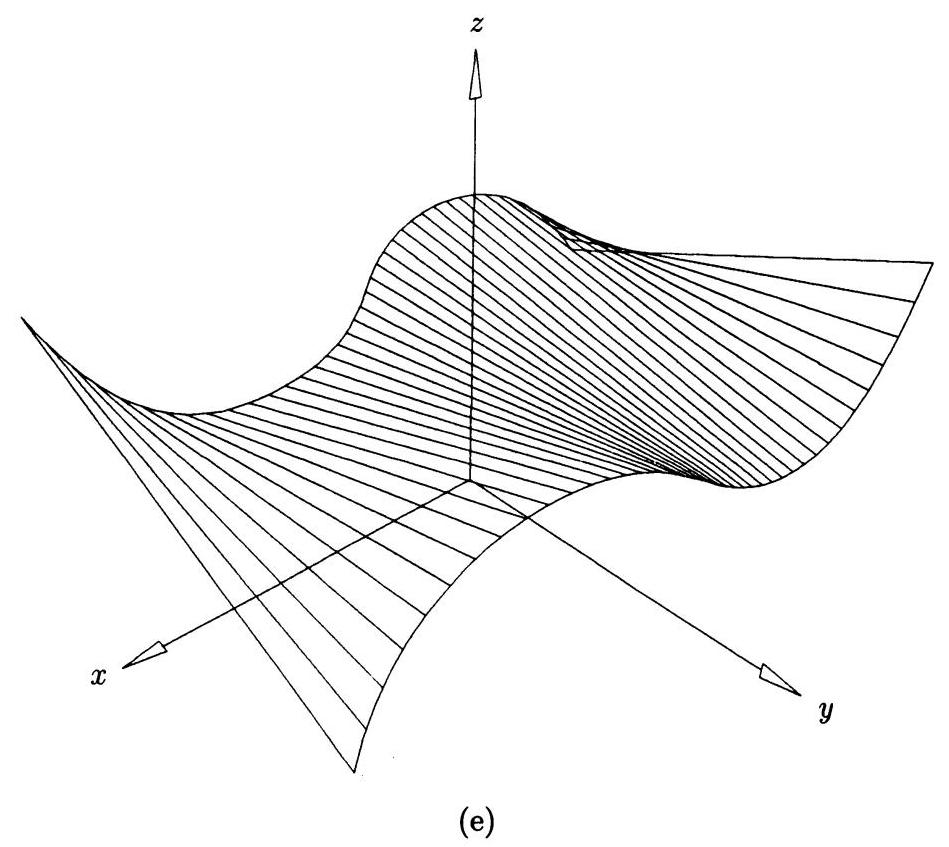
\includegraphics[max width=0.8\textwidth]{images/0193ba0d-ab19-7138-9798-cb281ce60de0_348_298_250_949_847_0.jpg}
\end{center}
\hspace*{3em} 

图 8.5. (续) (e) 规则曲面。

\begin{center}
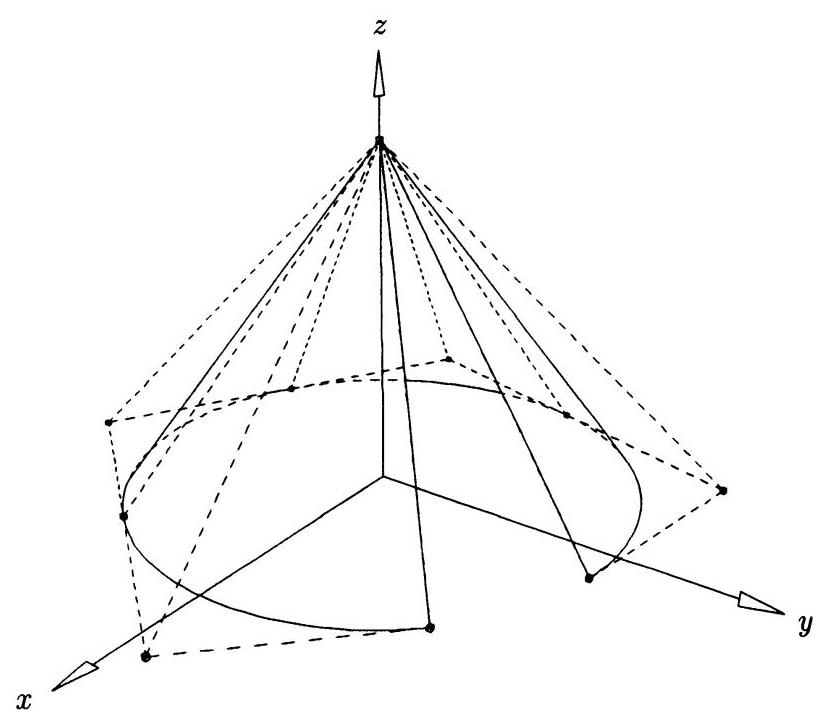
\includegraphics[max width=0.7\textwidth]{images/0193ba0d-ab19-7138-9798-cb281ce60de0_348_355_1338_826_723_0.jpg}
\end{center}
\hspace*{3em} 

图 8.6. 一个右圆锥面片。

\begin{center}
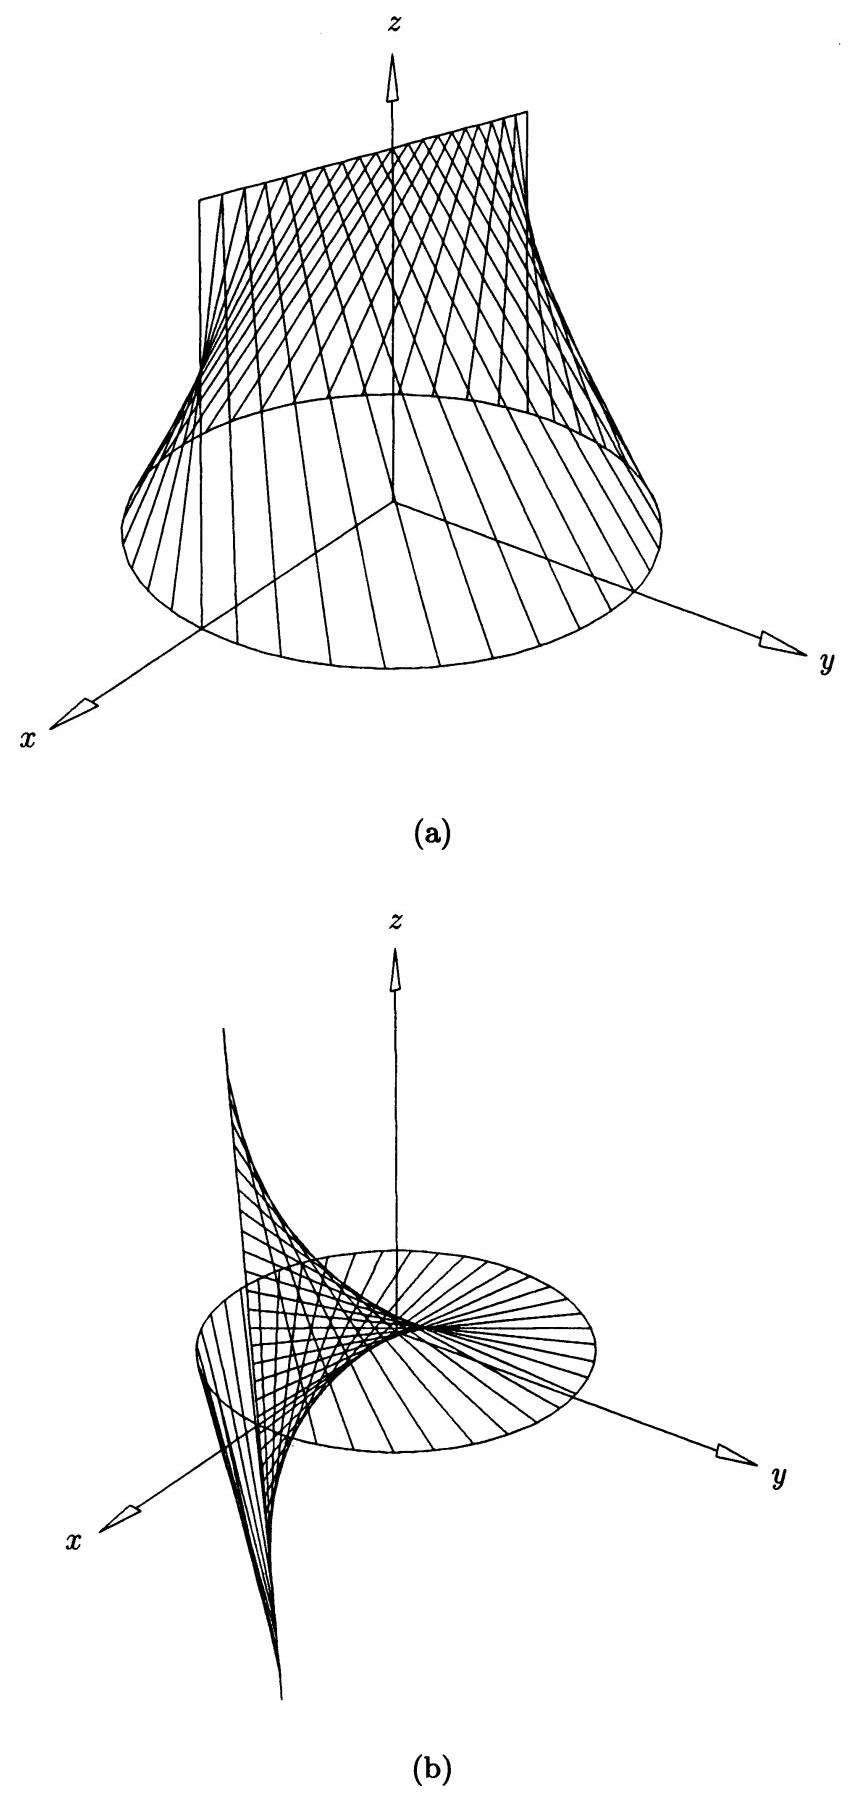
\includegraphics[max width=0.7\textwidth]{images/0193ba0d-ab19-7138-9798-cb281ce60de0_349_344_257_855_1794_0.jpg}
\end{center}
\hspace*{3em} 

图 8.7. 由圆和直线定义的规则曲面。 (a) 二阶规则曲面(圆锥面)；(b) 三阶规则曲面。

\begin{center}
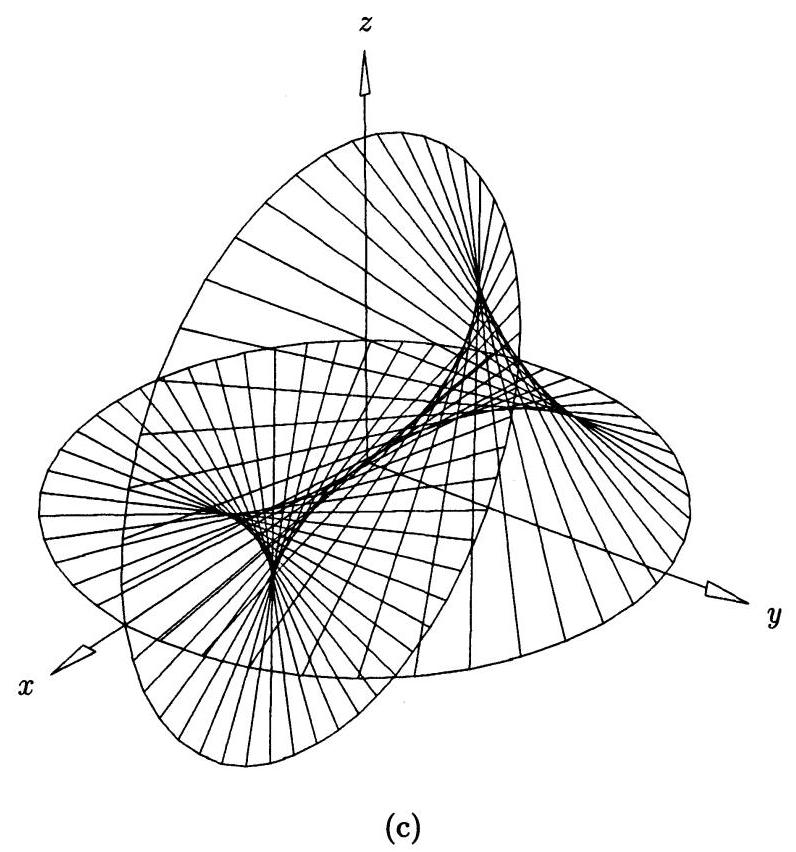
\includegraphics[max width=0.7\textwidth]{images/0193ba0d-ab19-7138-9798-cb281ce60de0_350_371_239_796_852_0.jpg}
\end{center}
\hspace*{3em} 

图 8.7. (续) (c) 四阶规则曲面。

\begin{center}
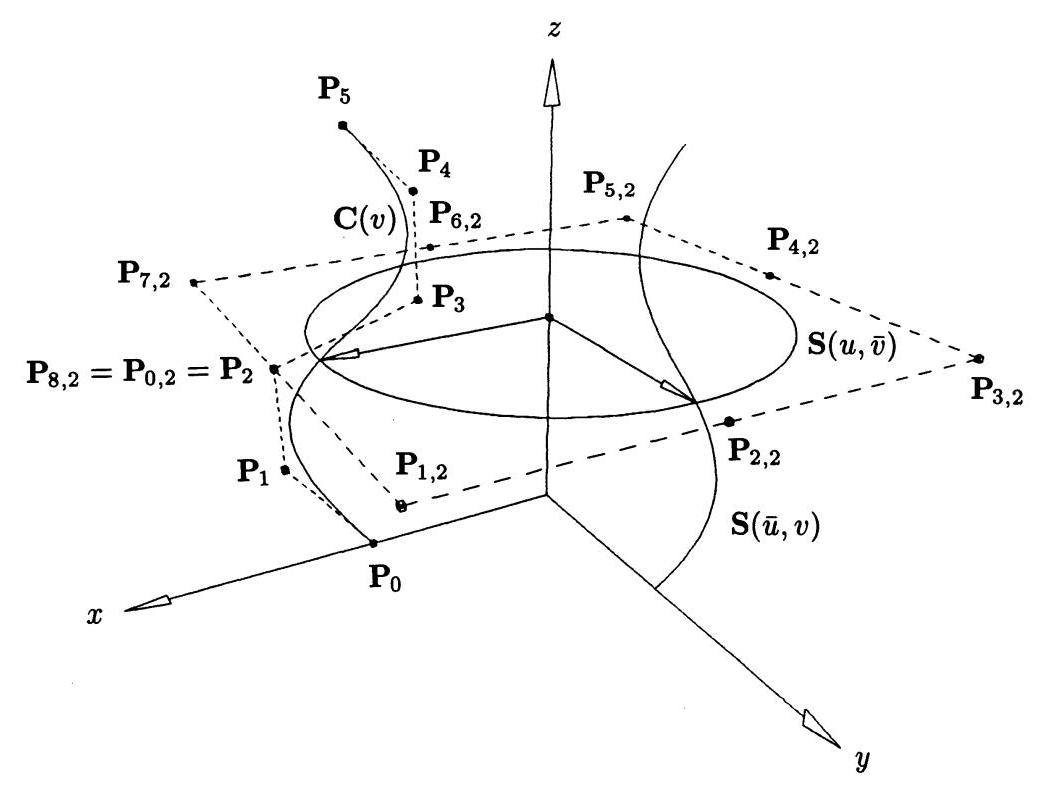
\includegraphics[max width=0.9\textwidth]{images/0193ba0d-ab19-7138-9798-cb281ce60de0_350_242_1280_1040_785_0.jpg}
\end{center}
\hspace*{3em} 

图 8.8. 旋转曲面的定义。

\begin{itemize}
\item 对于固定的 \(\bar{u},\mathbf{S}\left( {\bar{u},v}\right)\) ，曲线 \(\mathbf{C}\left( v\right)\) 绕 \(z\) 轴旋转一定角度；
\end{itemize}

\begin{itemize}
\item 对于固定的 \(\bar{v},\mathbf{S}\left( {u,\bar{v}}\right)\) ，是一个完整的圆，位于与 \(z\) 轴垂直的平面内，其中心在 \(z\) 轴上。
\end{itemize}

让我们使用九点圆表示法，带有 \(U = \left\{  {0,0,0,{1}^{\prime }{/}_{4},{1}_{/2},{1}_{/2}}\right.\) 、 \(\left. {3/4,3/4,1,1,1}\right\}\) 和权重 \({w}_{i} = \left\{  {1,\sqrt{2}/2,1,\sqrt{2}/2,1,\sqrt{2}/2,1,\sqrt{2}/2,1}\right\}\) 。然后所需的曲面具有以下形式

\[
\mathbf{S}\left( {u,v}\right)  = \mathop{\sum }\limits_{{i = 0}}^{8}\mathop{\sum }\limits_{{j = 0}}^{m}{R}_{i,2;j,q}\left( {u,v}\right) {\mathbf{P}}_{i,j} \tag{8.5}
\]

节点向量为 \(U\) 和 \(V\) 。控制点和权重的确定如下(见图 8.8):对于 \(i = 0,{\mathbf{P}}_{i,j} = {\mathbf{P}}_{0,j} = {\mathbf{P}}_{j}\) 。由于 \(\mathbf{S}\left( {u,\bar{v}}\right)\) 的循环特性，固定 \(j,0 \leq  i \leq  8\) 时，所有点都位于平面 \(z = {z}_{j}\) 中。它们位于宽度为 \(2{x}_{j}\) 的正方形上，中心在 \(z\) 轴上。权重通过取 \({w}_{j}\) 和圆形权重 \({w}_{i}\) 的乘积来定义，即，对于固定 \(j,{w}_{0,j} = {w}_{j},{w}_{1,j} = \left( {\sqrt{2}/2}\right) {w}_{j},{w}_{2,j} = {w}_{j},{w}_{3,j} = \left( {\sqrt{2}/2}\right) {w}_{j},\ldots ,{w}_{8,j} = {w}_{j}\) 。图 8.9a 和 \({8.9}\mathrm{\;b}\) 显示了控制网和由方程 (8.5) 生成的相应旋转曲面，以及图 8.8 的曲线。

并不完全明显方程 (8.5) 表示所需的旋转曲面，因此我们在此简要说明一个证明。固定 \(u = \bar{u}\) 并使用方程 (8.5) 的未投影形式，我们写道

\[
{\mathbf{S}}^{w}\left( {\bar{u},v}\right)  = \mathop{\sum }\limits_{{j = 0}}^{m}{N}_{j,q}\left( v\right) \left( {\mathop{\sum }\limits_{{i = 0}}^{8}{N}_{i,2}\left( \bar{u}\right) {\mathbf{P}}_{i,j}^{w}}\right)  = \mathop{\sum }\limits_{{j = 0}}^{m}{N}_{j,q}\left( v\right) {\mathbf{Q}}_{j}^{w}
\]

其中

\[
{\mathbf{Q}}_{j}^{w} = \mathop{\sum }\limits_{{i = 0}}^{8}{N}_{i,2}\left( \bar{u}\right) {\mathbf{P}}_{i,j}^{w}\;0 \leq  j \leq  m
\]

但这表明 \({\mathbf{Q}}_{j}\) 只是 \({\mathbf{P}}_{0,j}\left( { = {\mathbf{P}}_{j}}\right)\) 绕 \(z\) 轴旋转某个固定角度 \(\theta\) ，对应于 \(\bar{u}\) 。因此，由于 NURBS 曲线的旋转不变性，可以得出 \(\mathbf{S}\left( {\bar{u},v}\right)\) 只是 \(\mathbf{C}\left( v\right)\) 绕 \(z\) 轴旋转 \(\theta\) 。这完成了证明。

几种常见的表面是旋转表面。通过围绕 \(z\) 轴旋转一个完整的圆，可以得到一个环面(图 8.10)。通过围绕 \(z\) 轴旋转一个端点位于 \(z\) 轴上的半圆，可以得到一个球体(见图 8.11)。注意，球体的南北极的控制点重复了九次: \({\mathbf{P}}_{0,0} = \cdots  = {\mathbf{P}}_{8,0}\) 和 \({\mathbf{P}}_{0,4} = \cdots  = {\mathbf{P}}_{8,4}\) 。因此，这些极点关于 \(u\) 的偏导数是恒等于零的。然而，法向量在这些点显然是存在的。

我们现在提出一个算法，该算法通过任意角度 theta 绕任意轴构造 NURBS 旋转曲面(见图 8.12)。该轴由一个点 S 和一个单位长度向量 T 指定。为了方便，我们在这个算法中将权重和三维控制点分开；m, Pj[], wj[] 定义生成曲线，而 n, U, Pij[][] 被计算(见公式 [8.5])。我们假设有四个实用函数:

\begin{center}
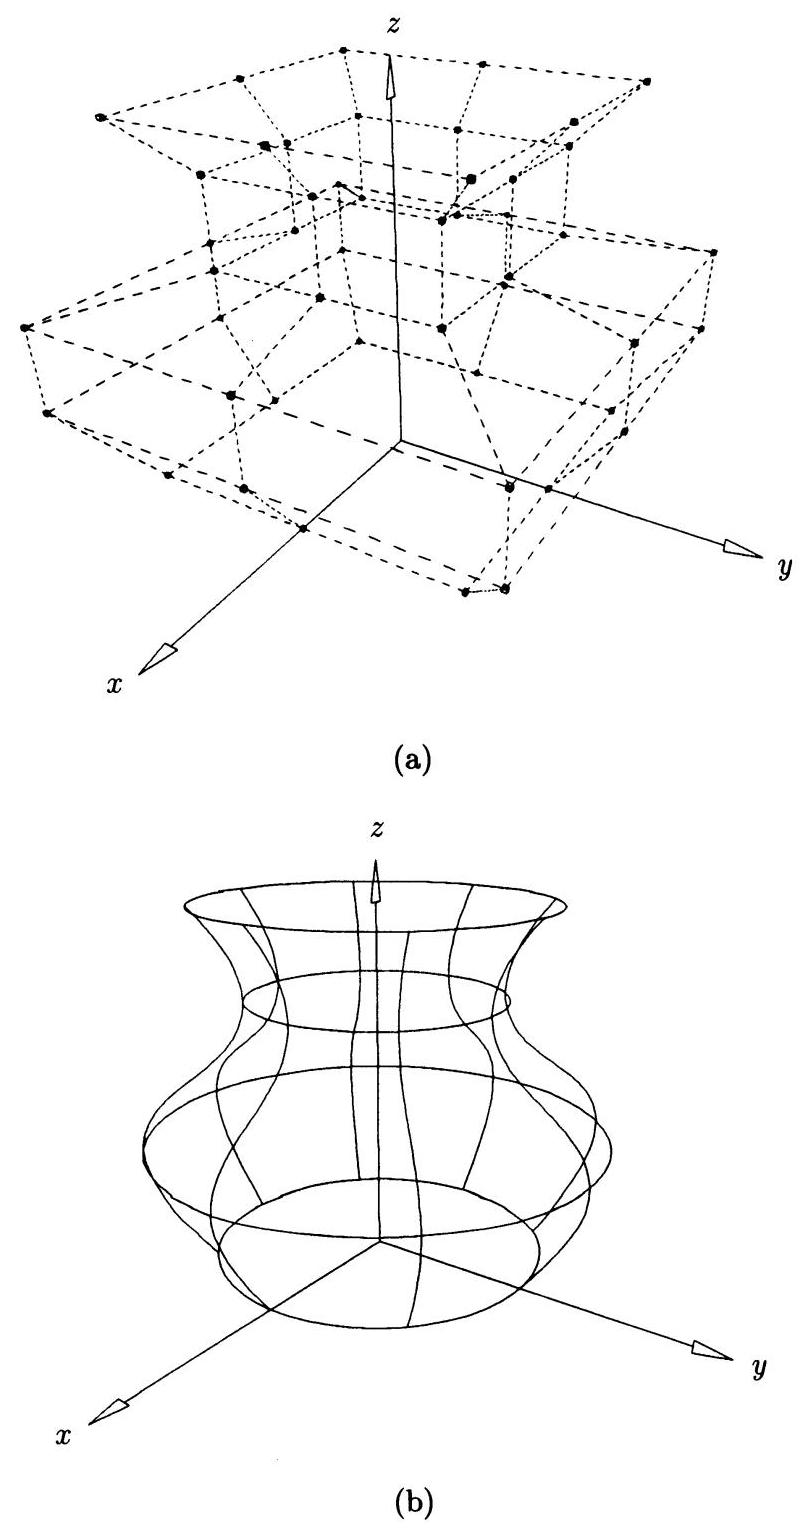
\includegraphics[max width=0.7\textwidth]{images/0193ba0d-ab19-7138-9798-cb281ce60de0_352_362_253_808_1532_0.jpg}
\end{center}
\hspace*{3em} 

图 8.9. (a.) 一个旋转表面的控制网；(b) 一个旋转表面。

PointToLine(   ) : 将一个点投影到一条线上；

VecNormalize(   ) : 归一化一个向量并返回其大小；

VecCrossProd(   ) : 计算向量的叉积；

Intersect3DLines (   ) : 交叉两条三维线。

注意这个算法与算法 A7.1 之间的相似性。346 常见表面的构造 算法 A8.1

\begin{center}
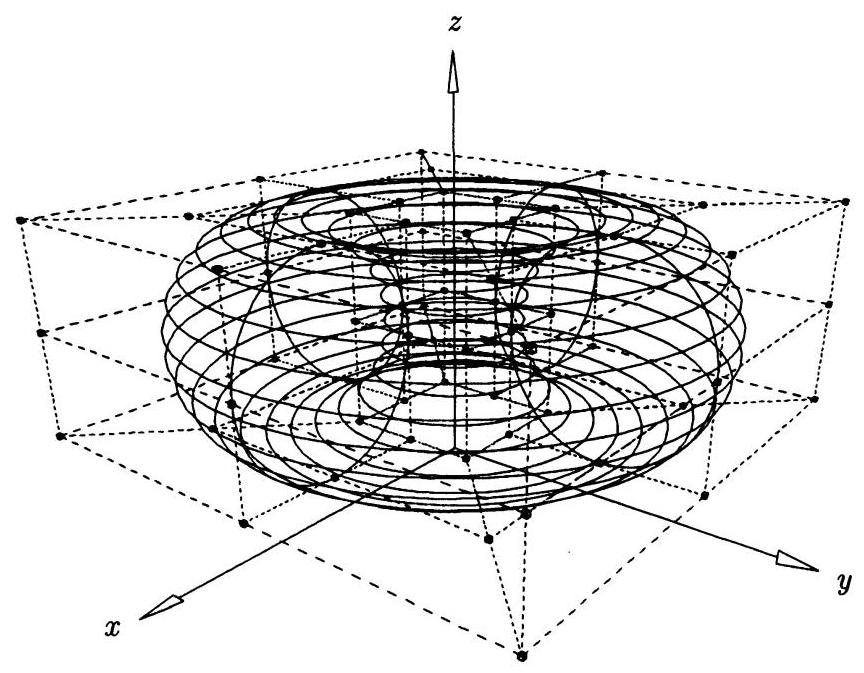
\includegraphics[max width=0.7\textwidth]{images/0193ba0d-ab19-7138-9798-cb281ce60de0_353_426_253_864_673_0.jpg}
\end{center}
\hspace*{3em} 

图 8.10. 作为旋转表面的环面。

\HRule

MakeRevolvedSurf (S, T, theta, m, Pj, wj, n, U, Pij, wij)

\hspace*{3em} \{ /* Create NURBS surface of revolution */

\hspace*{6em} /* Input: S, T, theta, m, Pj, wj */

\hspace*{6em} /* Output: n, U, Pij, wij */

\hspace*{2em} if (theta <= 90.0) narcs = 1 ;

\hspace*{5em} else

\hspace*{7em} if (theta <= 180.0)

\hspace*{10em} \{ narcs = 2; U[3] = U[4] = 0.5; \}

\hspace*{10em} else

\hspace*{12em} if (theta <= 270.0)

\hspace*{14em} \{

\hspace*{14em} narcs = 3 ;

\hspace*{14em} \(\mathrm{U}\left\lbrack  3\right\rbrack   = \mathrm{U}\left\lbrack  4\right\rbrack   = {1.0}/{3.0};\)

\hspace*{14em} U[5] = U[6] = 2.0/3.0;

\hspace*{14em} \}

\hspace*{14em} else

\hspace*{14em} \{

\hspace*{14em} narcs = 4 ;

\hspace*{14em} U[3] = U[4] = 0.25 ;

\hspace*{14em} U[5] = U[6] = 0.5 ;

\hspace*{14em} U[7] = U[8] = 0.75 ;

\hspace*{14em} \}

\hspace*{2em} dtheta = theta/narcs;

\hspace*{2em} j = 3 + 2*(narcs-1); /* load end knots */

\hspace*{2em} for (i=0; i<3; j++, i++)

\HRule

\begin{center}
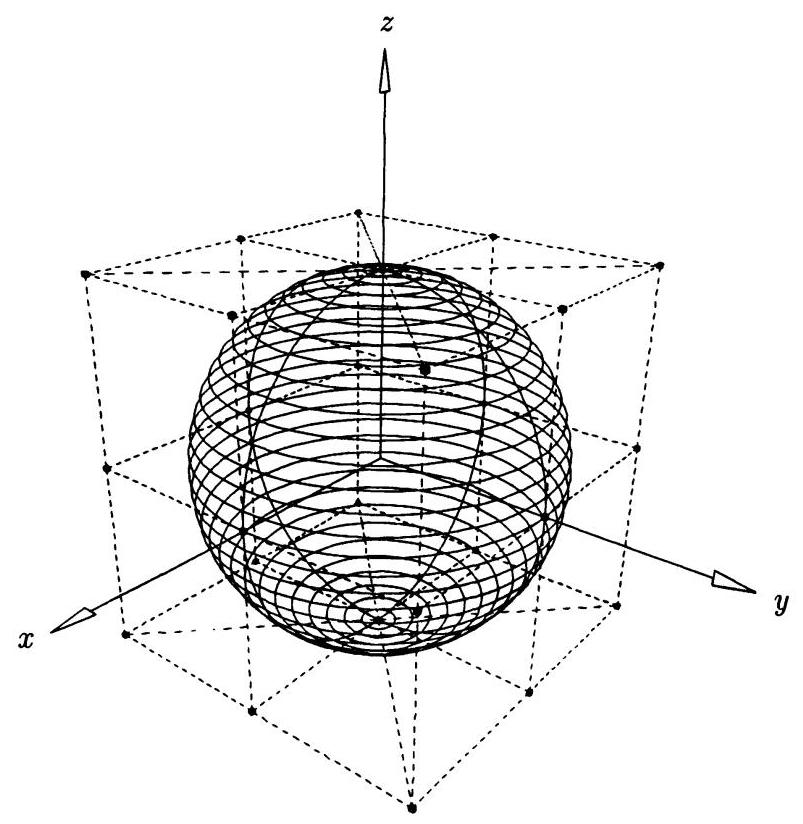
\includegraphics[max width=0.7\textwidth]{images/0193ba0d-ab19-7138-9798-cb281ce60de0_354_364_250_803_824_0.jpg}
\end{center}
\hspace*{3em} 

图 8.11. 作为旋转表面的球体。

\begin{center}
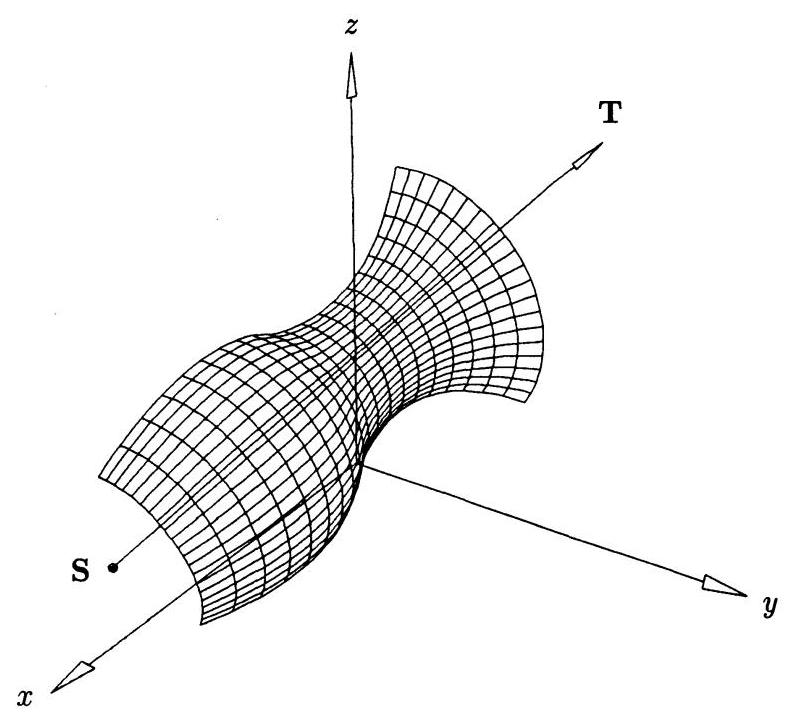
\includegraphics[max width=0.7\textwidth]{images/0193ba0d-ab19-7138-9798-cb281ce60de0_354_369_1307_794_720_0.jpg}
\end{center}
\hspace*{3em} 

图 8.12. 绕任意轴通过任意角度的通用旋转表面。

\HRule

\hspace*{1em} \(\left\{  {\;\mathrm{U}\left\lbrack  \mathrm{i}\right\rbrack   = {0.0};\;\mathrm{U}\left\lbrack  \mathrm{j}\right\rbrack   = {1.0};\;}\right\}\)

n = 2*narcs;

wm = cos(dtheta/2.0); /* dtheta/2 is base angle */

angle \(= {0.0};\;/ *\) Compute sines and cosines only once \(* /\)

for (i=1; i<=narcs; i++)

\hspace*{2em} \{

\hspace*{1em} angle = angle + dtheta;

\hspace*{2em} cosines[i] = cos(angle);

\hspace*{2em} sines[i] = sin(angle);

\hspace*{1em} \}

for (j=0; j<=m; j++)

\hspace*{2em} /* Loop and compute each \(u\) row of ctrl pts and weights \(*\) /

\hspace*{1em} \{

\hspace*{1em} PointToLine(S, T, Pj[j],0);

\hspace*{1em} \(X = {Pj}\left\lbrack  j\right\rbrack   - 0\) ;

\hspace*{1em} r = VecNormalize(X); VecCrossProd(T, X, Y);

\hspace*{1em} Pij[0][j] = P0 = Pj[j]; /* Initialize first */

\hspace*{1em} wij[0][j] = wj[j]; /* ctrl pt and weight */

\hspace*{2em} TO = Y; index = 0; angle = 0.0 ;

\hspace*{2em} for (i=1; i<=narcs; i++) /* compute u row */

\hspace*{3em} \{

\hspace*{3em} P2 = 0 + r*cosines[i]*X + r*sines[i]*Y;

\hspace*{3em} Pij[index+2][j] = P2;

\hspace*{3em} wij[index+2][j] = wj[j];

\hspace*{3em} T2 = -sines[i]*X + cosines[i]*Y;

\hspace*{3em} Intersect3DLines(PO, TO, P2, T2, Pij[index+1][j]);

\hspace*{3em} wij[index+1][j] = wm*wj[j];

\hspace*{3em} index = index + 2 ;

\hspace*{3em} if (i < narcs) \{ P0 = P2 ; T0 = T2 ; \}

\hspace*{3em} \}

\hspace*{1em} \}

\}

\HRule

图 8.13 显示了一个一般的环形补丁，作为一个旋转曲面，用于圆滑尖锐的角落。



\section{曲面的非均匀缩放}
设 \(\mathbf{P} = \left( {p}_{i}\right) ,i = 1,2,3\) 为三维空间中的一个点，设 \(F = \left( {f}_{i}\right)\) 、 \(i = 1,2,3\) 为三个实数(缩放因子)，分别对应每个坐标。关于原点按因子 \(F\) 进行缩放 \(\mathbf{P}\) 得到的点为

\[
\overline{\mathbf{P}} = \left( {\bar{p}}_{i}\right) \;{\bar{p}}_{i} = {f}_{i}{p}_{i},i = 1,2,3 \tag{8.6}
\]

如果 \(\mathbf{C} = \left( {c}_{i}\right)\) 是一个任意点，则 \(\mathbf{P}\) 通过方程在 \(\mathbf{C}\) 周围进行缩放。

\[
\overline{\mathbf{P}} = \left( {\bar{p}}_{i}\right) \;{\bar{p}}_{i} = {f}_{i}{p}_{i} + \left( {1 - {f}_{i}}\right) {c}_{i},i = 1,2,3 \tag{8.7}
\]

如果三个 \({f}_{i}\) 相等，则称缩放为均匀；否则，它是非均匀的。

通过对旋转曲面应用非均匀缩放，可以获得几个有趣的曲面。图 8.14 显示了一个以原点为中心的椭球，其隐式方程为

\[
\frac{{x}^{2}}{{a}^{2}} + \frac{{y}^{2}}{{b}^{2}} + \frac{{z}^{2}}{{c}^{2}} = 1 \tag{8.8}
\]

三个坐标平面将曲面切割成三个椭圆。椭球的构造是首先生成一个以原点为中心的单位半径球体，然后按因子 \(F = \left( {a,b,c}\right)\) 在原点周围进行缩放。

图 8.15b 显示了一个椭圆抛物面。 \({xz}\) 和 \({yz}\) 平面将曲面切割成抛物线； \({xy}\) 平面将其切割成一个椭圆。它的隐式方程为

\[
\frac{{x}^{2}}{{a}^{2}} + \frac{{y}^{2}}{{b}^{2}} = {cz} \tag{8.9}
\]

图 \({8.15}\mathrm{\;b}\) 的椭圆抛物面是通过对图 \({8.15}\mathrm{a}\) 中显示的旋转抛物面在原点周围按因子 \(F =\) (a, b,1) 进行缩放得到的。

通过将缩放因子应用于三维控制点，对 NURBS 曲面进行非均匀缩放。如果控制点存储在 350 常见曲面的构造中

\begin{center}
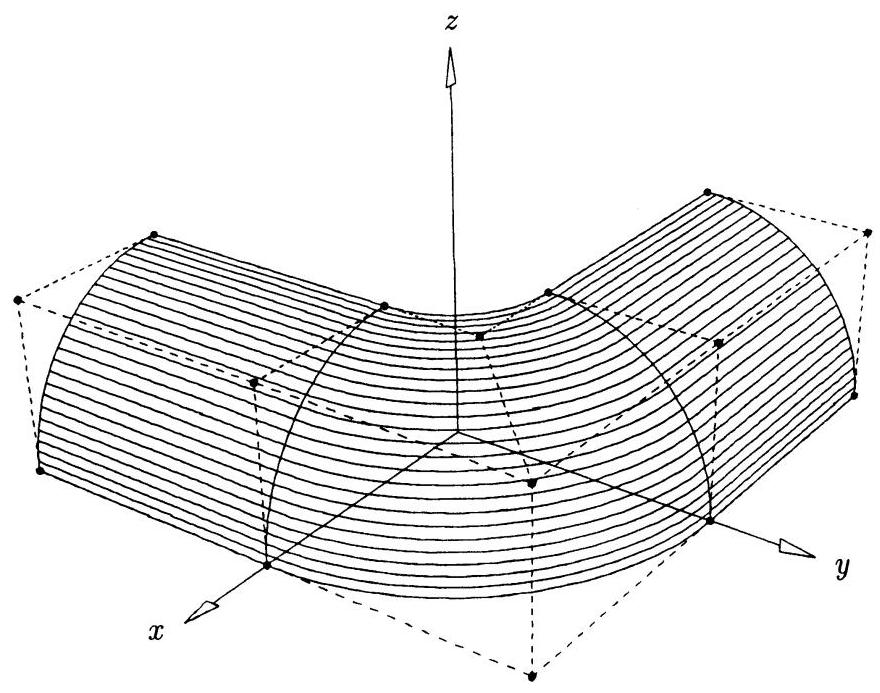
\includegraphics[max width=0.8\textwidth]{images/0193ba0d-ab19-7138-9798-cb281ce60de0_356_325_1374_880_693_0.jpg}
\end{center}
\hspace*{3em} 

图 8.13. 一个环形补丁作为旋转曲面，用于圆滑尖锐的角落。

\begin{center}
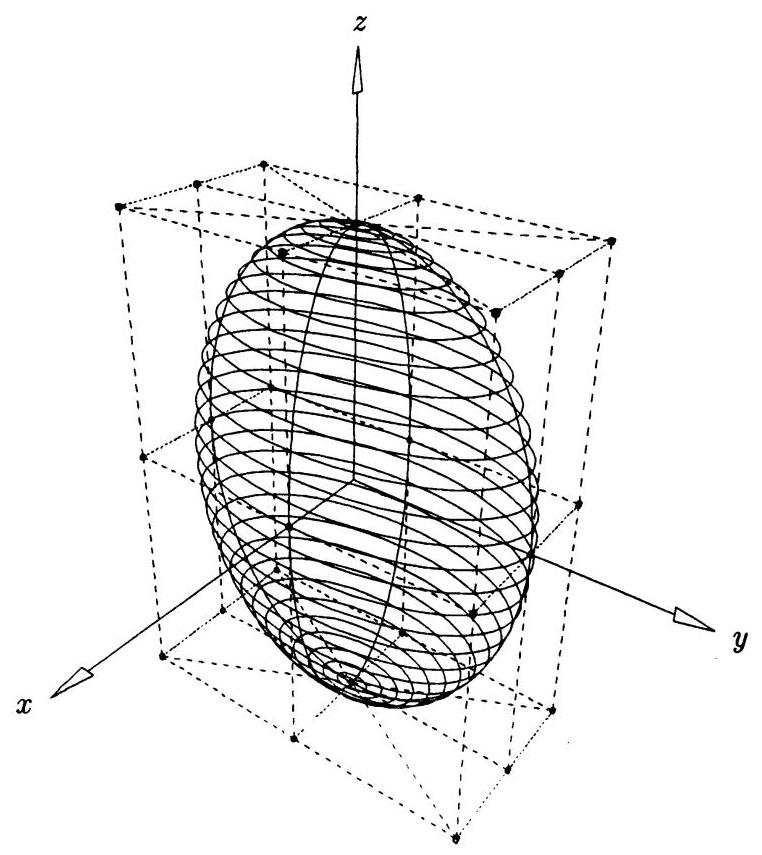
\includegraphics[max width=0.7\textwidth]{images/0193ba0d-ab19-7138-9798-cb281ce60de0_357_413_250_762_855_0.jpg}
\end{center}
\hspace*{3em} 

图 8.14. 通过缩放一个球体得到的椭球体。

\begin{center}
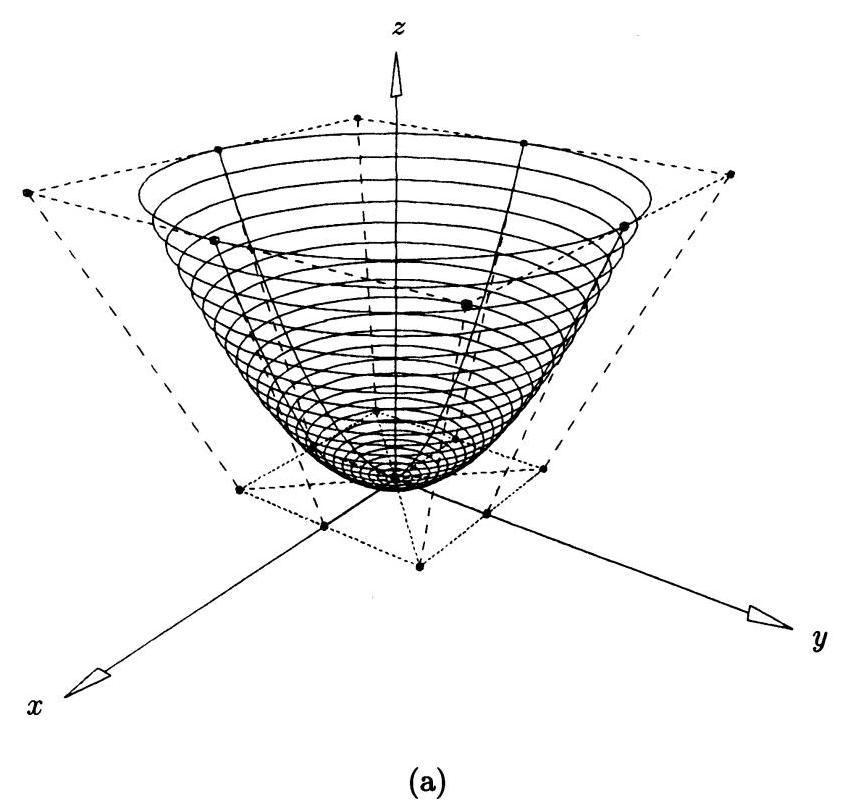
\includegraphics[max width=0.7\textwidth]{images/0193ba0d-ab19-7138-9798-cb281ce60de0_357_367_1305_843_802_0.jpg}
\end{center}
\hspace*{3em} 

图 8.15. 抛物面。(a) 旋转抛物面；(b) 椭圆抛物面。

\begin{center}
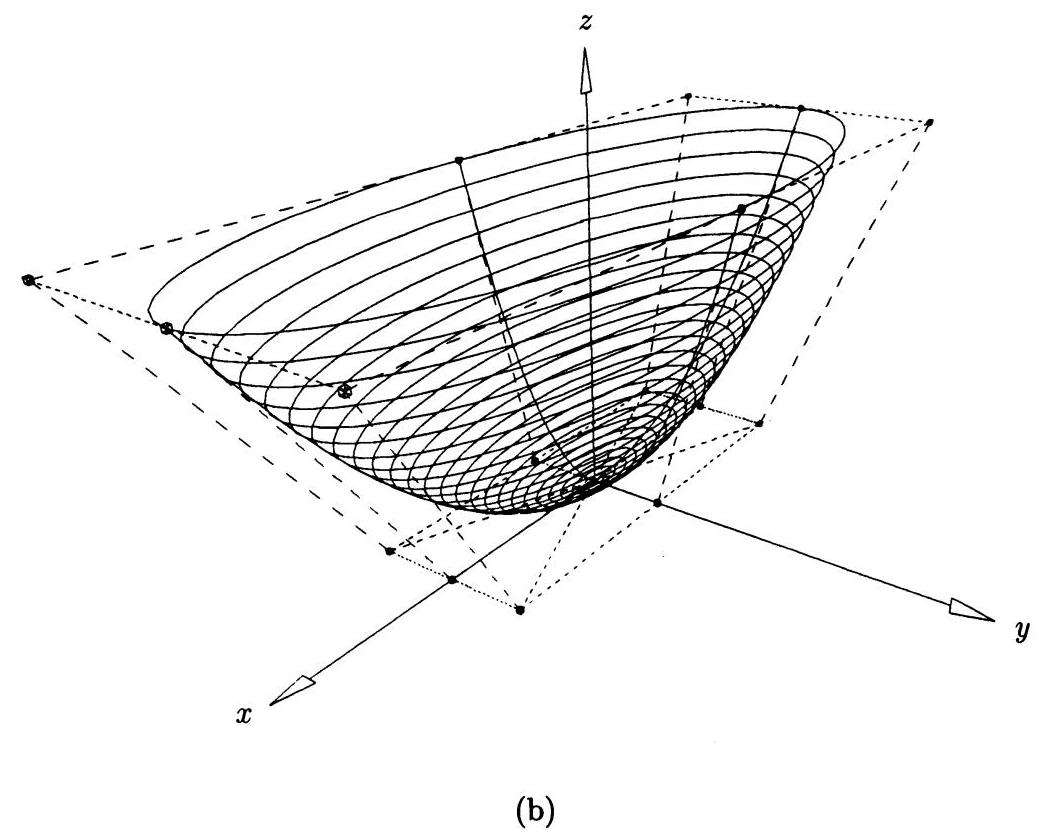
\includegraphics[max width=0.9\textwidth]{images/0193ba0d-ab19-7138-9798-cb281ce60de0_358_236_250_1039_837_0.jpg}
\end{center}
\hspace*{3em} 

图 8.15. (续。)

在三维(无权重)形式下，则可以直接应用公式 (8.6) 或公式 (8.7)。权重不变。如果控制点以四维形式存储

\[
{\mathbf{P}}^{w} = \left( {{p}_{1}^{w},{p}_{2}^{w},{p}_{3}^{w},w}\right)  = \left( {{p}_{i}^{w},w}\right) \;i = 1,2,3
\]

则只有前三个坐标会发生变化。公式 (8.6) 变为

\[
{\overline{\mathbf{P}}}^{w} = \left( {{\bar{p}}_{i}^{w},w}\right) \;{\bar{p}}_{i}^{w} = {f}_{i}{p}_{i}^{w},i = 1,2,3 \tag{8.10}
\]

公式 (8.7) 变为

\[
{\overline{\mathbf{P}}}^{w} = \left( {{\bar{p}}_{i}^{w},w}\right) \;{\bar{p}}_{i}^{w} = {f}_{i}{p}_{i}^{w} + \left( {1 - {f}_{i}}\right) w{c}_{i},i = 1,2,3 \tag{8.11}
\]



\section{三边球面}
当三个表面相交时，结果是三条边缘曲线在一个角点相遇(见图8.16a)。由于在制造零件中，尖锐的边缘和角通常是不受欢迎的，因此需要一些“平滑”或“圆滑”尖锐边缘和角的表面。这些被称为圆角表面。获得圆角表面的一个常见概念方法是滚动弹珠模型。如果一个半径为 \(R\) 的弹珠沿着所有边缘曲线滚动并进入角落，则会得到图 \({8.16}\mathrm{\;b}\) 的表面 \({\mathbf{S}}_{4} - {\mathbf{S}}_{7}\) 。 \({\mathbf{S}}_{4} - {\mathbf{S}}_{6}\) 是边缘圆角，而 \({\mathbf{S}}_{7}\) 是一个角落 352 常见表面的圆角。与各自边缘曲线方向垂直的 \({\mathbf{S}}_{4} - {\mathbf{S}}_{6}\) 的横截面是半径为 \(R\) 的圆弧，其弧长随着表面沿边缘的角度变化而变化。一般来说，这些表面相当复杂，无法精确表示为 NURBS 形式。使用 NURBS 时，通常在用户指定的容差范围内进行近似。角落圆角 \({\mathbf{S}}_{7}\) 是一个三边补丁，位于半径为 \(R\) 的球体上。我们使用“补丁”一词来表示某个更大表面的子表面。三个边界曲线是半径为 \(R\) 的圆弧，其中心与球体的中心重合。此外，假设表面不相切，弧的扫角小于 \({180}^{ \circ  }\) ，因此每个弧都可以用一个所有权重为正的 Bézier 段表示。角落圆角可以精确表示为一个 \(\left( {4 \times  2}\right)\) 次 NURBS 表面，具有一个退化边界。

除了获得角落圆角表面外，这里提出的方法是构造二次曲面上张量积补丁的更一般技术的一个简单特例。二次曲面是任何具有以下形式的二阶隐式方程的表面

\[
S\left( {x,y,z}\right)  = a{x}^{2} + b{y}^{2} + c{z}^{2} + {dxy} + {exz} + {fyz} + {gx} + {hy} + {iz} + j = 0 \tag{8.12}
\]

球体、椭球体、双曲面、抛物面，以及圆柱体和圆锥体是二次曲面的例子。所有这些，以及许多其他重要的曲面，如环面和生成曲线为二次的旋转曲面，都是由两组最大度数为2的曲线生成的。例如，球体是由两组圆(纬线和经线)生成的，而右圆柱体则由一组直线和一组圆生成。如果补丁边界曲线是由这两组生成曲线组成的曲线的部分，则可以使用第8.2-8.6节中的技术在这些曲面上构建补丁。生成的曲面补丁是双二次的。如果补丁边界不遵循生成曲线(如一般角落圆角的情况)，那么情况会更复杂，补丁甚至可能无法表示为NURBS曲面。对于底层曲面为二次且补丁边界为圆锥截面的情况，已经获得了一些结果和算法，例如，见[Geis90; Boeh91; Hosc92a]。

现在我们展示如何构建角落圆角。尽管细节相当复杂，但该方法在概念上相当简单；我们只是组合两个映射。为了不失一般性，我们假设底层球体的半径为 \(R\) ，并且位于(0,0, R)(见图8.17)。众所周知的立体投影 \(\textit{projection (see [Coxe67; DoCa76]) yields a rational parametric representation of}\) 球体 \({\mathbf{S}}_{1}\left( {u,v}\right)  = \left( {x\left( {u,v}\right) ,y\left( {u,v}\right) ,z\left( {u,v}\right) }\right)\) ，其中

\[
x\left( {u,v}\right)  = \frac{4{R}^{2}u}{{u}^{2} + {v}^{2} + 4{R}^{2}}
\]

\[
y\left( {u,v}\right)  = \frac{4{R}^{2}v}{{u}^{2} + {v}^{2} + 4{R}^{2}}
\]

\[
z\left( {u,v}\right)  = \frac{{2R}\left( {{u}^{2} + {v}^{2}}\right) }{{u}^{2} + {v}^{2} + 4{R}^{2}} \tag{8.13}
\]

即，a(u, v)点映射到(x, y, z)点，该点位于球体与从(u, v,0)到(0,0,2R)的线段的交点(见图8.17)。在此投影下，我们有以下对应关系:

\begin{center}
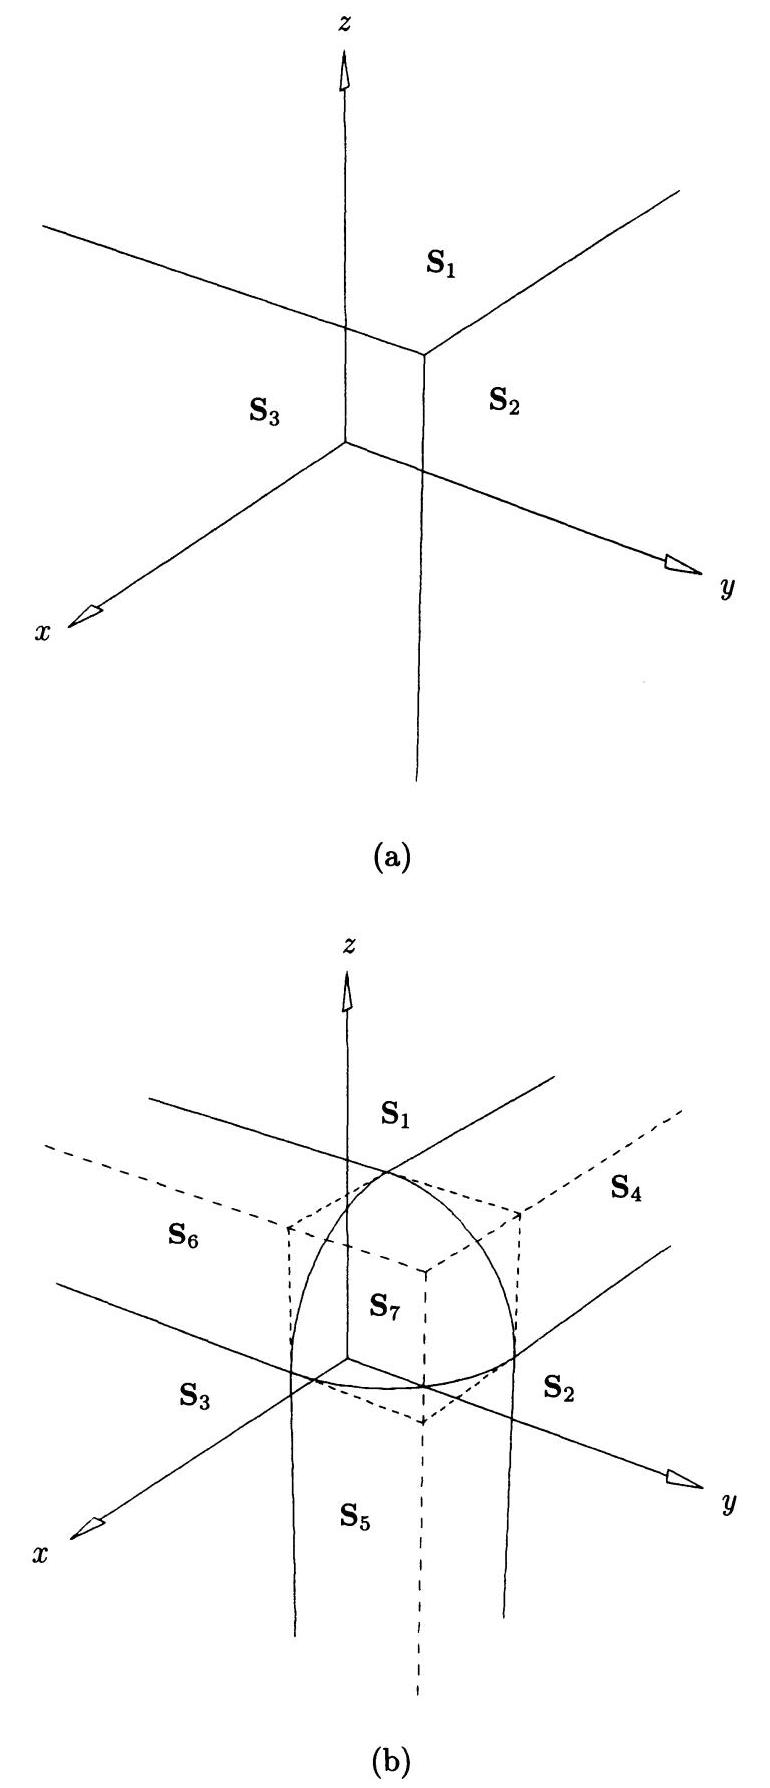
\includegraphics[max width=0.7\textwidth]{images/0193ba0d-ab19-7138-9798-cb281ce60de0_360_383_252_770_1788_0.jpg}
\end{center}
\hspace*{3em} 

图 8.16. 圆角和一个角落。(a) 由三条相交平面形成的三条边和一个角落；(b) 通过滚动一个弹珠形成的三条边缘圆角面和一个角落圆角面；圆角和三条边缘以虚线表示。

\begin{itemize}
\item 通过 \({xy}\) 平面原点的直线映射到球体上的经线圆；
\end{itemize}

\begin{itemize}
\item 球体上的所有其他圆对应于 \({xy}\) 平面上的圆。
\end{itemize}

圆角表面的三个边界是半径为 \(R\) 的圆弧，中心在 (0,0, R) 处。将这些弧记作 \({\mathbf{C}}_{1}\left( t\right) ,{\mathbf{C}}_{2}\left( s\right) ,{\mathbf{C}}_{3}\left( t\right)\) ，其中 \(0 \leq  s,t \leq  1\) 。为了不失一般性，我们假设补丁边界的位置和方向如下(见图 8.18):

\begin{itemize}
\item \({\mathbf{C}}_{1}\left( t\right)\) 和 \({\mathbf{C}}_{3}\left( t\right)\) 从原点开始: \({\mathbf{C}}_{1}\left( 0\right)  = {\mathbf{C}}_{3}\left( 0\right)  = \left( {0,0,0}\right)\) ；
\end{itemize}

\begin{itemize}
\item \({\mathbf{C}}_{1}\left( t\right)\) 位于 \({xz}\) 平面内；
\end{itemize}

\begin{itemize}
\item \({\mathbf{C}}_{1}\left( 1\right)  = {\mathbf{C}}_{2}\left( 0\right)\) 和 \({\mathbf{C}}_{2}\left( 1\right)  = {\mathbf{C}}_{3}\left( 1\right)\) 。
\end{itemize}

然后，圆角补丁的投影产生一个平面， \({\mathbf{S}}_{2}\left( {s,t}\right)  = (u\left( {s,t}\right)\) ， \(v\left( {s,t}\right) ,0)\) 在 \({xy}\) 平面内。 \(s = 0\) 和 \(s = 1\) 的边界是直线， \(t = 0\) 边界是退化的，而 \(t = 1\) 边界是一个圆弧。因此， \({\mathbf{S}}_{2}\left( {s,t}\right)\) 的度数为 (2,1)，而复合映射 \(\mathbf{S}\left( {s,t}\right)  = {\mathbf{S}}_{1} \circ  {\mathbf{S}}_{2}\) 产生了一个 \(\left( {4 \times  2}\right)\) 度的有理 Bézier 表示。

显然，可以推导出计算 \(\mathbf{S}\left( {s,t}\right)\) 的控制点和权重的一般公式。然而，由于大多数项本身为零，我们特别为每个坐标和权重分别推导公式。计算过程为:

\begin{center}
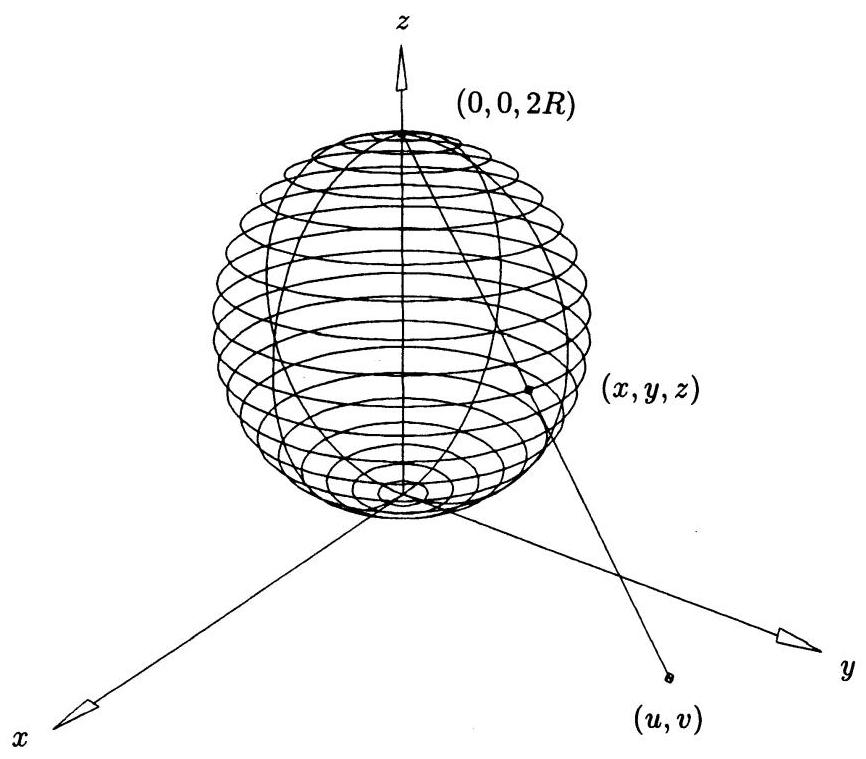
\includegraphics[max width=0.7\textwidth]{images/0193ba0d-ab19-7138-9798-cb281ce60de0_361_330_1331_866_759_0.jpg}
\end{center}
\hspace*{3em} 

图 8.17. 立体投影。

\begin{center}
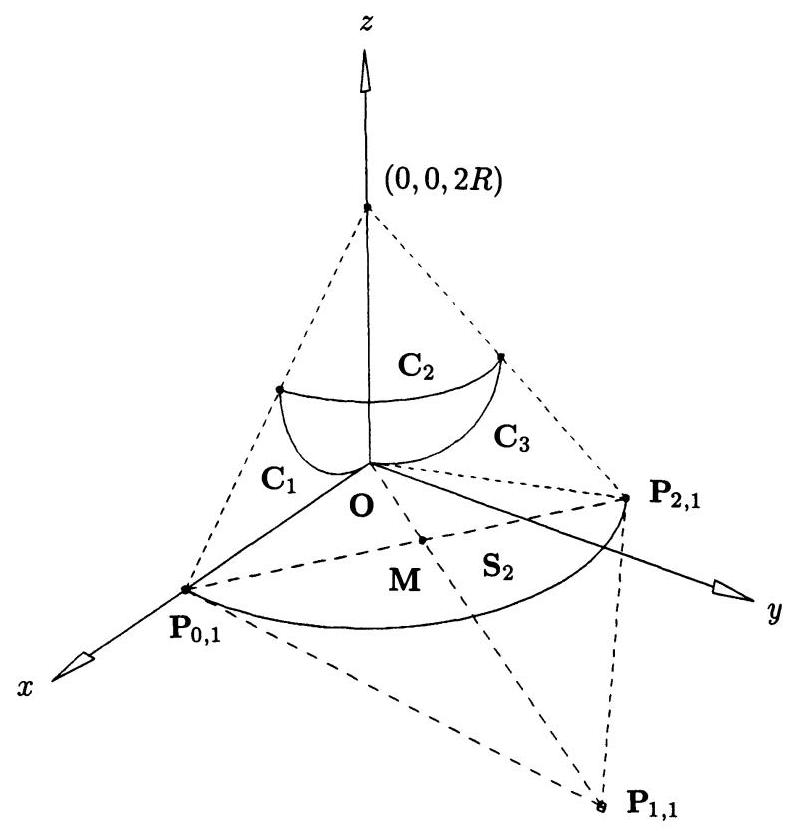
\includegraphics[max width=0.7\textwidth]{images/0193ba0d-ab19-7138-9798-cb281ce60de0_362_369_252_797_831_0.jpg}
\end{center}
\hspace*{3em} 

图 8.18. 通过将圆角表面投影到 \({xy}\) 平面上获得的平面 \({\mathbf{S}}_{2}\) 。

1. 获取 \({\mathbf{S}}_{2}\left( {s,t}\right)\) 的贝塞尔表示；

2. 将 \({\mathbf{S}}_{2}\left( {s,t}\right)\) 转换为幂基形式；

3. 将 \({\mathbf{S}}_{2}\left( {s,t}\right)\) 的幂基系数代入 \({\mathbf{S}}_{1}\left( {u,v}\right)\) (方程 [8.13]) 以获得圆角补丁的幂基形式 \(\mathbf{S}\left( {s,t}\right)\) ；

4. 将 \(\mathbf{S}\left( {s,t}\right)\) 转换为贝塞尔形式。

\({\mathbf{S}}_{2}\left( {s,t}\right)\) 的贝塞尔表示需要六个四维控制点 \({\mathbf{P}}_{i,j}^{w},0 \leq  i \leq  2,0 \leq  j \leq  1\) 。显然， \({\mathbf{P}}_{0,0} = {\mathbf{P}}_{1,0} = {\mathbf{P}}_{2,0} = \left( {0,0,0}\right)\) ，其中 \({w}_{0,0} = {w}_{2,0} = 1.{w}_{1,0}\) 被设定为等于 \({w}_{1,1}\) ，这仍需稍后计算。 \({\mathbf{P}}_{i,1}^{w},0 \leq  i \leq  2\) 是圆弧的控制点，它是 \({\mathbf{C}}_{2}\left( s\right)\) 的投影。它们的获取方法如下:

1. 将三点 \({\mathbf{C}}_{2}\left( 0\right) ,{\mathbf{C}}_{2}\left( {1/2}\right)\) 和 \({\mathbf{C}}_{2}\left( 1\right)\) 投影到 \({xy}\) 平面中的圆弧上。设 (x, y, z) 为这些点之一的坐标；则投影的 \({uv}\) 坐标通过公式计算得出。

\[
\alpha  = \frac{-{2R}}{z - {2R}}\;u = {\alpha x},v = {\alpha y} \tag{8.14}
\]

这得到了 \({\mathbf{P}}_{0,1}^{w}\) 和 \({\mathbf{P}}_{2,1}^{w}\left( {{w}_{0,1} = {w}_{2,1} = 1}\right)\) 。

2. 计算投影弧的中心 (图 8.18 中的 O) 和半径 \(r\) ；例如，通过交叉三点 \({\mathbf{C}}_{2}\left( 0\right)\) 、 \({\mathbf{C}}_{2}\left( {1/2}\right)\) 和 \({\mathbf{C}}_{2}\left( 1\right)\) 投影形成的两条弦的垂直平分线找到 \(\mathbf{O}\) ；

3. 然后通过 (见图 8.18) 计算 \({\mathbf{P}}_{1,1}^{w}\) :

\begin{itemize}
\item 计算 \(\mathbf{M} = 1/2\left( {{\mathbf{P}}_{0,1} + {\mathbf{P}}_{2,1}}\right)\) ；
\end{itemize}

\begin{itemize}
\item \({\mathbf{P}}_{1,1}\) 是关于投影圆弧的 \(\mathbf{M}\) 的逆(见 [Coxe67])，因此 \(\mathbf{{OM}} \cdot  {\mathbf{{OP}}}_{1,1} = {r}^{2}\) ; 从中我们得到
\end{itemize}

\[
{\mathbf{P}}_{1,1} = \left( {1 - \alpha }\right) \mathbf{O} + \alpha \mathbf{M}
\]

其中

\[
\alpha  = \frac{{r}^{2}}{{\left| \mathbf{{OM}}\right| }^{2}}
\]

\begin{itemize}
\item 从方程 (7.33) 可得 \({w}_{1,1} = \cos \angle {\mathbf{P}}_{1,1}{\mathbf{P}}_{2,1}{\mathbf{P}}_{0,1}\) .
\end{itemize}

设 \(\left\lbrack  {\mathbf{a}}_{i,j}^{w}\right\rbrack\) 表示 \({\mathbf{S}}_{2}^{w}\left( {s,t}\right)\) 的幂基系数。从方程 (6.91) 可以得出

\[
\left\lbrack  {\mathbf{a}}_{i,j}^{w}\right\rbrack   = {M}_{2}\left\lbrack  {\mathbf{P}}_{i,j}^{w}\right\rbrack  {M}_{1}^{T}
\]

其中 \({M}_{2}\) 和 \({M}_{1}\) 分别是二阶和一阶贝塞尔矩阵(方程 [6.80])。应用矩阵乘法得到

\[
{\mathbf{a}}_{0,0}^{w} = {\mathbf{P}}_{0,0}^{w}
\]

\[
{\mathbf{a}}_{0,1}^{w} = {\mathbf{P}}_{0,1}^{w} - {\mathbf{P}}_{0,0}^{w}
\]

\[
{\mathbf{a}}_{1,0}^{w} = 2\left( {{\mathbf{P}}_{1,0}^{w} - {\mathbf{P}}_{0,0}^{w}}\right)
\]

\[
{\mathbf{a}}_{1,1}^{w} = 2\left( {{\mathbf{P}}_{1,1}^{w} + {\mathbf{P}}_{0,0}^{w} - {\mathbf{P}}_{0,1}^{w} - {\mathbf{P}}_{1,0}^{w}}\right)
\]

\[
{\mathbf{a}}_{2,0}^{w} = {\mathbf{P}}_{0,0}^{w} - 2{\mathbf{P}}_{1,0}^{w} + {\mathbf{P}}_{2,0}^{w}
\]

\[
{\mathbf{a}}_{2,1}^{w} = {\mathbf{P}}_{0,1}^{w} + {\mathbf{P}}_{2,1}^{w} - {\mathbf{P}}_{0,0}^{w} - {\mathbf{P}}_{2,0}^{w} + 2\left( {{\mathbf{P}}_{1,0}^{w} - {\mathbf{P}}_{1,1}^{w}}\right)  \tag{8.15}
\]

现在设

\[
{\mathbf{a}}_{i,j}^{w} = \left( {{u}_{i,j},{v}_{i,j},{h}_{i,j}}\right)  \tag{8.16}
\]

(注意 \({u}_{i,j}\) 和 \({v}_{i,j}\) 是加权的)。 \(z\) 坐标为零，为了避免后续的冲突，我们使用 \(h\) 代替 \(w\) 作为权重。将圆弧的控制点表示为 \({\mathbf{P}}_{i,1}^{w} = \left( {{\alpha }_{i},{\beta }_{i},{\gamma }_{i}}\right) ,0 \leq  i \leq  2\left( {\alpha }_{i}\right.\) 和 \(\left. {\beta }_{i}\right)\) 加权 \()\) 。假设角权重为 1，并考虑到 \({\mathbf{C}}_{1}\left( t\right)\) 位于 \({xz}\) 平面且 \({\mathbf{C}}_{1}\left( 0\right)  = \left( {0,0,0}\right)\) ，可以得出唯一非零的 \({u}_{i,j},{v}_{i,j}\) 和 \({h}_{i,j}\) 是

\[
{u}_{0,1} = {\alpha }_{0}
\]

\[
{u}_{1,1} = 2\left( {{\alpha }_{1} - {\alpha }_{0}}\right)
\]

\[
{u}_{2,1} = {\alpha }_{2} + {\alpha }_{0} - 2{\alpha }_{1}
\]

\[
{v}_{1,1} = 2{\beta }_{1}
\]

\[
{v}_{2,1} = {\beta }_{2} - 2{\beta }_{1}
\]

\[
{h}_{0,0} = 1
\]

\[
{h}_{1,0} = 2\left( {{\gamma }_{1} - 1}\right)
\]

\[
{h}_{2,0} = 2\left( {1 - {\gamma }_{1}}\right)  \tag{8.17}
\]

使用方程 (8.16) 和 (8.17) 以及幂基形式

我们得到

\[
{\mathbf{S}}_{2}^{w}\left( {s,t}\right)  = \left\lbrack  \begin{array}{lll} 1 & s & {s}^{2} \end{array}\right\rbrack  \left\lbrack  {\mathbf{a}}_{i,j}^{w}\right\rbrack  \left\lbrack  \begin{array}{l} 1 \\  t \end{array}\right\rbrack   \tag{8.18}
\]

\[
{\mathbf{S}}_{2}\left( {s,t}\right)  = \left( {u\left( {s,t}\right) ,v\left( {s,t}\right) }\right)
\]

其中

\[
u\left( {s,t}\right)  = \frac{U\left( {s,t}\right) }{H\left( {s,t}\right) }\;v\left( {s,t}\right)  = \frac{V\left( {s,t}\right) }{H\left( {s,t}\right) } \tag{8.19}
\]

和

\[
U\left( {s,t}\right)  = {u}_{0,1}t + {u}_{1,1}{st} + {u}_{2,1}{s}^{2}t
\]

\[
V\left( {s,t}\right)  = {v}_{1,1}{st} + {v}_{2,1}{s}^{2}t
\]

\[
H\left( {s,t}\right)  = {h}_{0,0} + {h}_{1,0}s + {h}_{2,0}{s}^{2} \tag{8.20}
\]

将方程 (8.19) 和 (8.20) 代入方程 (8.13)，我们得到

\[
\mathbf{S}\left( {s,t}\right)  = \left( {x\left( {s,t}\right) ,y\left( {s,t}\right) ,z\left( {s,t}\right) }\right)  \tag{8.21}
\]

\[
x\left( {s,t}\right)  = \frac{X\left( {s,t}\right) }{W\left( {s,t}\right) }\;y\left( {s,t}\right)  = \frac{Y\left( {s,t}\right) }{W\left( {s,t}\right) }\;z\left( {s,t}\right)  = \frac{Z\left( {s,t}\right) }{W\left( {s,t}\right) } \tag{8.22}
\]

和 \(X\left( {s,t}\right)  = 4{R}^{2}U\left( {s,t}\right) H\left( {s,t}\right)\)

\[
= 4{R}^{2}\left( {{u}_{0,1}t + {u}_{1,1}{st} + {u}_{2,1}{s}^{2}t}\right) \left( {{h}_{0,0} + {h}_{1,0}s + {h}_{2,0}{s}^{2}}\right)
\]

\[
= 4{R}^{2}\left\lbrack  {{u}_{0,1}{h}_{0,0}t + \left( {{u}_{1,1}{h}_{0,0} + {u}_{0,1}{h}_{1,0}}\right) {st}}\right.
\]

\[
+ \left( {{u}_{2,1}{h}_{0,0} + {u}_{1,1}{h}_{1,0} + {u}_{0,1}{h}_{2,0}}\right) {s}^{2}t
\]

\[
\left. {+\left( {{u}_{2,1}{h}_{1,0} + {u}_{1,1}{h}_{2,0}}\right) {s}^{3}t + {u}_{2,1}{h}_{2,0}{s}^{4}t}\right\rbrack   \tag{8.23}
\]

\[
Y\left( {s,t}\right)  = 4{R}^{2}V\left( {s,t}\right) H\left( {s,t}\right)
\]

\[
= 4{R}^{2}\left( {{v}_{1,1}{st} + {v}_{2,1}{s}^{2}t}\right) \left( {{h}_{0,0} + {h}_{1,0}s + {h}_{2,0}{s}^{2}}\right)
\]

\[
= 4{R}^{2}\lbrack {v}_{1,1}{h}_{0,0}{st} + \left( {{v}_{2,1}{h}_{0,0} + {v}_{1,1}{h}_{1,0}}\right) {s}^{2}t
\]

\[
+ \left( {{v}_{1,1}{h}_{2,0} + {v}_{2,1}{h}_{1,0}}\right) {s}^{3}t + {v}_{2,1}{h}_{2,0}{s}^{4}t\rbrack  \tag{8.24}
\]

\[
Z\left( {s,t}\right)  = {2R}\left\lbrack  {U{\left( s,t\right) }^{2} + V{\left( s,t\right) }^{2}}\right\rbrack
\]

\[
= {2R}\left\lbrack  {{u}_{0,1}^{2}{t}^{2} + 2{u}_{0,1}{u}_{1,1}s{t}^{2} + \left( {{u}_{1,1}^{2} + 2{u}_{0,1}{u}_{2,1} + {v}_{1,1}^{2}}\right) {s}^{2}{t}^{2}}\right.
\]

\[
\left. {+2\left( {{u}_{1,1}{u}_{2,1} + {v}_{1,1}{v}_{2,1}}\right) {s}^{3}{t}^{2} + \left( {{u}_{2,1}^{2} + {v}_{2,1}^{2}}\right) {s}^{4}{t}^{2}}\right\rbrack   \tag{8.25}
\]

\[
W\left( {s,t}\right)  = U{\left( s,t\right) }^{2} + V{\left( s,t\right) }^{2} + 4{R}^{2}H{\left( s,t\right) }^{2}
\]

\[
= 4{R}^{2}{h}_{0,0}^{2} + 8{R}^{2}{h}_{0,0}{h}_{1,0}s + 4{R}^{2}\left( {{h}_{1,0}^{2} + 2{h}_{0,0}{h}_{2,0}}\right) {s}^{2} + {u}_{0,1}^{2}{t}^{2}
\]

\[
+ 8{R}^{2}{h}_{1,0}{h}_{2,0}{s}^{3} + 2{u}_{0,1}{u}_{1,1}s{t}^{2} + 4{R}^{2}{h}_{2,0}^{2}{s}^{4}
\]

\[
+ \left( {{u}_{1,1}^{2} + 2{u}_{0,1}{u}_{2,1} + {v}_{1,1}^{2}}\right) {s}^{2}{t}^{2}
\]

\[
+ 2\left( {{u}_{1,1}{u}_{2,1} + {v}_{1,1}{v}_{2,1}}\right) {s}^{3}{t}^{2} + \left( {{u}_{2,1}^{2} + {v}_{2,1}^{2}}\right) {s}^{4}{t}^{2} \tag{8.26}
\]

记作

\[
{\mathbf{S}}^{w}\left( {s,t}\right)  = \left\lbrack  {s}^{i}\right\rbrack  \left\lbrack  {\mathbf{b}}_{i,j}^{w}\right\rbrack  {\left\lbrack  {t}^{j}\right\rbrack  }^{T}\;0 \leq  i \leq  4\;0 \leq  j \leq  2 \tag{8.27}
\]

\({\mathbf{S}}^{w}\left( {s,t}\right)\) 的幂基表示，并设 \({\mathbf{b}}_{i,j}^{w} = \left( {{x}_{i,j},{y}_{i,j},{z}_{i,j},{w}_{i,j}}\right)\) 。 \({\mathbf{b}}_{i,j}^{w}\) 的大多数坐标为零。唯一的非零元素是

\[
{x}_{0,1} = 4{R}^{2}{u}_{0,1}{h}_{0,0}
\]

\[
{x}_{1,1} = 4{R}^{2}\left( {{u}_{1,1}{h}_{0,0} + {u}_{0,1}{h}_{1,0}}\right)
\]

\[
{x}_{2,1} = 4{R}^{2}\left( {{u}_{2,1}{h}_{0,0} + {u}_{1,1}{h}_{1,0} + {u}_{0,1}{h}_{2,0}}\right)
\]

\[
{x}_{3,1} = 4{R}^{2}\left( {{u}_{2,1}{h}_{1,0} + {u}_{1,1}{h}_{2,0}}\right)
\]

\[
{x}_{4,1} = 4{R}^{2}{u}_{2,1}{h}_{2,0} \tag{8.28}
\]

\[
{y}_{1,1} = 4{R}^{2}{v}_{1,1}{h}_{0,0}
\]

\[
{y}_{2,1} = 4{R}^{2}\left( {{v}_{2,1}{h}_{0,0} + {v}_{1,1}{h}_{1,0}}\right)
\]

\[
{y}_{3,1} = 4{R}^{2}\left( {{v}_{1,1}{h}_{2,0} + {v}_{2,1}{h}_{1,0}}\right)
\]

\[
{y}_{4,1} = 4{R}^{2}{v}_{2,1}{h}_{2,0} \tag{8.29}
\]

\[
{z}_{0,2} = {2R}{u}_{0,1}^{2}
\]

\[
{z}_{1,2} = {4R}{u}_{0,1}{u}_{1,1}
\]

\[
{z}_{2,2} = {2R}\left( {{u}_{1,1}^{2} + 2{u}_{0,1}{u}_{2,1} + {v}_{1,1}^{2}}\right)
\]

\[
{z}_{3,2} = {4R}\left( {{u}_{1,1}{u}_{2,1} + {v}_{1,1}{v}_{2,1}}\right)
\]

\[
{z}_{4,2} = {2R}\left( {{u}_{2,1}^{2} + {v}_{2,1}^{2}}\right)  \tag{8.30}
\]

\[
{w}_{0,0} = 4{R}^{2}{h}_{0,0}^{2}
\]

\[
{w}_{1,0} = 8{R}^{2}{h}_{0,0}{h}_{1,0}
\]

\[
{w}_{2,0} = 4{R}^{2}\left( {{h}_{1,0}^{2} + 2{h}_{0,0}{h}_{2,0}}\right)
\]

\[
{w}_{3,0} = 8{R}^{2}{h}_{1,0}{h}_{2,0}
\]

\[
{w}_{4,0} = 4{R}^{2}{h}_{2,0}^{2}
\]

\[
{w}_{0,2} = {u}_{0,1}^{2}
\]

\[
{w}_{1,2} = 2{u}_{0,1}{u}_{1,1}
\]

\[
{w}_{2,2} = {u}_{1,1}^{2} + 2{u}_{0,1}{u}_{2,1} + {v}_{1,1}^{2}
\]

\[
{w}_{3,2} = 2\left( {{u}_{1,1}{u}_{2,1} + {v}_{1,1}{v}_{2,1}}\right)
\]

\[
{w}_{4,2} = {u}_{2,1}^{2} + {v}_{2,1}^{2} \tag{8.31}
\]

方程 (8.27)-(8.31) 给出了填角表面 \({\mathbf{S}}^{w}\left( {s,t}\right)\) 的幂基形式。通过应用方程 (6.100) 得到 Bézier (NURBS) 表示，即

\[
\left\lbrack  {\mathbf{P}}_{i,j}^{w}\right\rbrack   = {M}_{4}^{-1}\left\lbrack  {\mathbf{b}}_{i,j}^{w}\right\rbrack  {\left( {M}_{2}^{-1}\right) }^{T}
\]

算法 A6.2 用于计算 \({M}_{4}^{-1}\) 和 \({M}_{2}^{-1}\) 。

\begin{center}
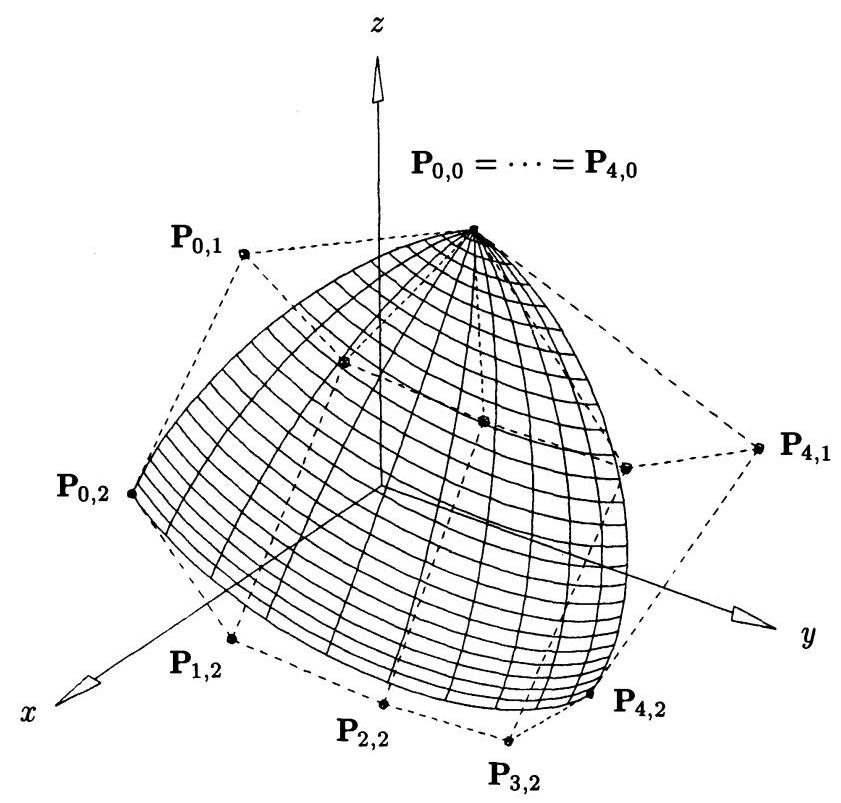
\includegraphics[max width=0.7\textwidth]{images/0193ba0d-ab19-7138-9798-cb281ce60de0_366_344_250_841_803_0.jpg}
\end{center}
\hspace*{3em} 

图 8.19。一个角落填角表面 - 一个任意的球面补丁，其边界是球体的大圆。

现在我们总结完整的算法。算法的输入是三个边界弧 \({\mathbf{C}}_{1},{\mathbf{C}}_{2}\) 和 \({\mathbf{C}}_{3}\) ，它们在空间中任意定位和定向，但在其端点处相连。输出是一个 \(\left( {4 \times  2}\right)\) 度的有理 Bézier 填角补丁。

算法 A8.2

MakeCornerFilletSurf (C1, C2, C3, Pwij)

\{ /* 创建 NURBS 角落填角表面 */

/* 输入: C1, C2, C3 */

/* 输出: Pwij */

1. 计算三个边界弧的公共半径和中心点。

2. 使用平移、旋转以及可能的曲线反转(见第6章)，将边界弧定位和定向，如图8.18所示。请注意，实际上只有 \({\mathbf{C}}_{2}\) 需要被定位和定向，因为只有它是计算三个控制点 \({\mathbf{P}}_{i,1}^{w} = \left( {{\alpha }_{i},{\beta }_{i},{\gamma }_{i}}\right) .\) 所必需的。

3. 按照上述描述计算 \(\left( {{\alpha }_{i},{\beta }_{i},{\gamma }_{i}}\right)\) 。

4. 将 \({\mathbf{S}}_{2}^{w}\left( {s,t}\right)\) 从贝塞尔形式转换为幂基形式(方程 [8.17])。

5. 计算圆角补丁 \({\mathbf{S}}^{w} = {\mathbf{S}}_{1}^{w} \circ  {\mathbf{S}}_{2}^{w}\) 的幂基形式(方程 [8.27] - [8.31])。

360 公共曲面的构造

6. 将 \({\mathbf{S}}^{w}\left( {s,t}\right)\) 转换为有理贝塞尔形式(方程 [8.32] 和算法 A6.2)。

7. 将 \(\mathbf{S}\left( {s,t}\right)\) 旋转/平移回三维空间中的正确位置(步骤2的逆变换)。

\}



\end{document}


